\documentclass[twoside,a5paper,11pt]{article}

\usepackage[top=1.1in,bottom=0.9in,left=1in,right=0.8in]{geometry}

\usepackage{fontspec, xunicode, xltxtra}  
\usepackage{xeCJK}

%\usepackage{geometry}                % See geometry.pdf to learn the layout options. There are lots.
%\geometry{letterpaper}                   % ... or a4paper or a5paper or ... 
%\geometry{landscape}                % Activate for for rotated page geometry
\usepackage[parfill]{parskip}    % Activate to begin paragraphs with an empty line rather than an indent
\usepackage{graphicx}
\usepackage{amssymb}
\usepackage{amsmath}
\usepackage{url}

\usepackage{mathrsfs}
\usepackage{imakeidx}

% Will Robertson's fontspec.sty can be used to simplify font choices.
% To experiment, open /Applications/Font Book to examine the fonts provided on Mac OS X,
% and change "Hoefler Text" to any of these choices.

\usepackage{fontspec,xltxtra,xunicode}
\defaultfontfeatures{Mapping=tex-text}
\setromanfont[Mapping=tex-text]{Hoefler Text}
\setsansfont[Scale=MatchLowercase,Mapping=tex-text]{Gill Sans}
\setmonofont[Scale=MatchLowercase]{Andale Mono}

\makeindex

%\setmainfont{Microsoft YaHei}  

\setmainfont{STKaiti}


\title{量子力学II}
\author{@季燕江}
\date{\today}                                           % Activate to display a given date or no date

\begin{document}

\pagestyle{headings}

\maketitle


\begin{abstract}

本讲稿(读书笔记)基于樱井教授所著的《现代量子力学》(J. J. Sakurai, Modern Quantum Mechanics, Revised Edition)。

\end{abstract}

\tableofcontents{1}

版本:1.0

GIT: \url{http://github.com/jiyanjiang/AQM2014}

豆瓣小站:\url{http://site.douban.com/223228/}

\section{斯特恩-盖拉赫实验}

有两种讲授量子力学的方式,一种是历史的方式,基本按时间次序交待上世纪量子力学创建过程中的关键进展,比如先介绍卢瑟福的散射实验,然后介绍普朗克的量子化,玻尔理论,进而讨论德布罗意的物质波概念,高潮部分是薛定谔的波动力学。

另一种是公理的方式,即用最少的实验事实建立量子力学的形式体系,引入狄拉克记号和矩阵力学。在量子力学II中我们将采用公理的方式讲授量子力学。这样讲授量子力学的好处是在数学上较清晰,方便我们后续发展种种方法系统地研究物理问题。

量子力学II和量子力学I研究的都是非相对论的单粒子问题,从物理内容上讲并无本质的增加。量子力学I多采用历史的方式讲授,大部分精力会花在波动力学上。而量子力学II会采用公理的方式讲授,它从一开始就要引入并使用狄拉克记号,主要使用矩阵力学(在历史上被认为比波动力学更抽象)讨论量子力学。

量子力学II的重点不在讨论物理学史上那些曾引发起无数争论和不可思议的实验,但完全不介绍实验事实也不可能,因为量子力学到底是一种物理理论,而非数学理论。费曼在其物理学讲义中通过双缝实验引入量子力学,而在樱井书中则是通过斯特恩-盖拉赫实验来引入量子力学的。

在双缝实验中我们很难接受粒子会像波一样行为,因为粒子在人们的日常经验中已经被强烈地规定了,我们很难把粒子想象为不像一块石头那样行为。但对斯特恩-盖拉赫实验而言就不存在这个“很难接受”的问题,因为我们本来叙述的就是一种非日常经验,我们只需把它当做一个黑盒子去想象就可以了。

通过斯特恩-盖拉赫实验会大大降低进入量子世界的门槛。

\subsection{斯特恩和盖拉赫}

斯特恩\index{Otto Stern:斯特恩}(Otto Stern)是学物理化学出身,犹太人,后来追随爱因斯坦学习理论物理,但其真正擅长的还是实验物理,斯特恩是最早发展分子束技术的科学家,他用这个方法直观地验证了气体分子确实是遵从麦克斯韦分布律的,并使用这个方法测定了银原子的磁矩,甚至是质子的磁矩等等。

1922年,他与盖拉赫\index{Walter Gerlach:盖拉赫}(Walter Gerlach)合作,完成了斯特恩-盖拉赫实验。斯特恩做这个实验的初始动机是要验证玻尔提出的空间量子化\index{Space quantization:空间量子化}(Space quantization)概念,即原子的磁矩只能取向于空间的分立方向上。当时人们认为原子磁矩来源于原子内部电子的轨道运动,电子延圆形或椭圆轨道围绕原子核运动就像环形电流一样会产生磁矩。空间量子化意味着这些圆形或椭圆轨道只能存在于特定空间取向的平面上。

但实际上斯特恩-盖拉赫实验\index{Stern-Gerlach experiment:斯特恩盖-拉赫实验}却揭示出电子本身就具有磁矩,如果我们称因轨道运动所导致的磁矩是轨道磁矩的话,这种新磁矩就称之为自旋磁矩,轨道磁矩对应轨道角动量,而自旋磁矩则对应自旋角动量。此前人们已经知道轨道角动量量子数是取整数的,而斯特恩-盖拉赫实验却显示自旋角动量量子数是半整数($1/2$)。这可以说是使物理学家大开眼界了,而且也完全超出实验的设计者斯特恩和盖拉赫的预想。

由于该实验在物理学史中的关键作用,斯特恩被授予1943年的诺贝尔物理奖(此前的1940,41,42正值二战最凶险的时刻,连续三年无人获奖,因斯特恩的犹太人身份,当时斯特恩已经逃到美国,并加入美国籍),而斯特恩本人则是被提名诺贝尔物理学奖次数最多的一位科学家,从1925-1943年他共获得了81次提名\footnote{Physicsworld.com, Nobel population 1901-50: anatomy of a scientific elite. \url{http://physicsworld.com/cws/article/print/2001/nov/05/nobel-population-1901-to-50-anatomy-of-a-scientific-elite}}。

有趣的是盖拉赫作为实验的关键合作者却未同时得奖,实际上盖拉赫在同时期也获得了30次提名,超过革末(Germer)、郎之万(Langevin)、外斯(Weiss)、梅特纳(Meitner)等同样未获得诺贝尔奖的著名物理学家的提名次数。但因德国“异议人士”卡尔·冯·奥西茨基1935年获得诺贝尔和平奖\footnote{当时奥西茨基正在服刑,纳粹德国不同意释放他去领奖,因此奥西茨基成为第一位在监狱里获得诺贝尔奖的人。\url{http://en.wikipedia.org/wiki/Carl_von_Ossietzky}},希特勒视之为对自己的羞辱,于1937年颁布法令禁止任何德国人领取任何诺贝尔奖,这使得正与纳粹合作的纯种日耳曼人盖拉赫很难有获奖的可能性。

\subsection{非均匀磁场}

实验的关键是“非均匀磁场”,斯特恩和盖拉赫制造了专门的具有特殊形状的磁铁,使得磁场基本就在$z$方向上,并且延$z$方向上是非均匀的:

\begin{eqnarray}
\vec B & =  & B_z \hat z \\
\frac{\partial }{\partial z} B_z & \neq & 0
\end{eqnarray}

我们把一个磁矩$\mu$放到磁场里,其能量是:

\begin{equation}
E(z) = - \mu \cdot B = - \mu_z B_z  
\end{equation}

磁矩\index{Magnetic moment:磁矩}在非均匀磁场里会受到一个$z$方向上的力:

\begin{equation}
F_z = - \frac{\partial E(z)}{\partial z} = \mu_z \frac{\partial B_z}{\partial z}
\end{equation}

$\mu_z$就是磁矩在$z$方向上的分量,实验采用的粒子是银原子\index{Silver atom:银原子},即把处于高温的银原子引出来,通过准直装置飞进非均匀磁场里。

\begin{figure}[htbp]
\begin{center}
\includegraphics[width=10cm]{SGExperiment/SGexperiment.png}
\caption{斯特恩-盖拉赫实验装置示意}
%\label{default}
\end{center}
\end{figure}

银原子的原子序数是47,其电子结构可表示为:$[Kr] 4 d^{10} 5s$。

现在考虑银原子的磁矩,首先原子核的磁矩远小于电子的磁矩,这意味着我们只需要考虑银原子中电子磁矩的贡献,其次以我们今天的知识原子中满壳层或满亚壳层电子磁矩的贡献正好互相抵消(轨道磁矩和自旋磁矩都会抵消),这样我们就可判定银原子的磁矩主要来自$5s$电子的贡献。

对$s$轨道而言,轨道角动量为0,这样电子的轨道磁矩也没有了,唯一有贡献的就是$5s$电子的自旋磁矩,换句话说银原子就其磁学性质而言,它就是一个自旋$1/2$的小磁针(银原子束将分裂为上、下两束),只不过它比较重,远重于单电子的质量。

根据银原子束分裂的大小,我们可以把银原子的磁矩表示为:

\begin{equation}
\mu_z = - \frac{e}{2m } s_z
\end{equation}

这里$m$表示电子的质量,而$s_z = \pm \frac{1}{2} \hbar$,即银原子磁矩的取值有两种可能性,一正一负,或说延$z$方向一上一下,相应地银原子在非均匀磁场里的受力也是两种,延$z$方向的一上一下。这就解释了银原子在非均匀磁场里的分裂。

\begin{figure}[htbp]
\begin{center}
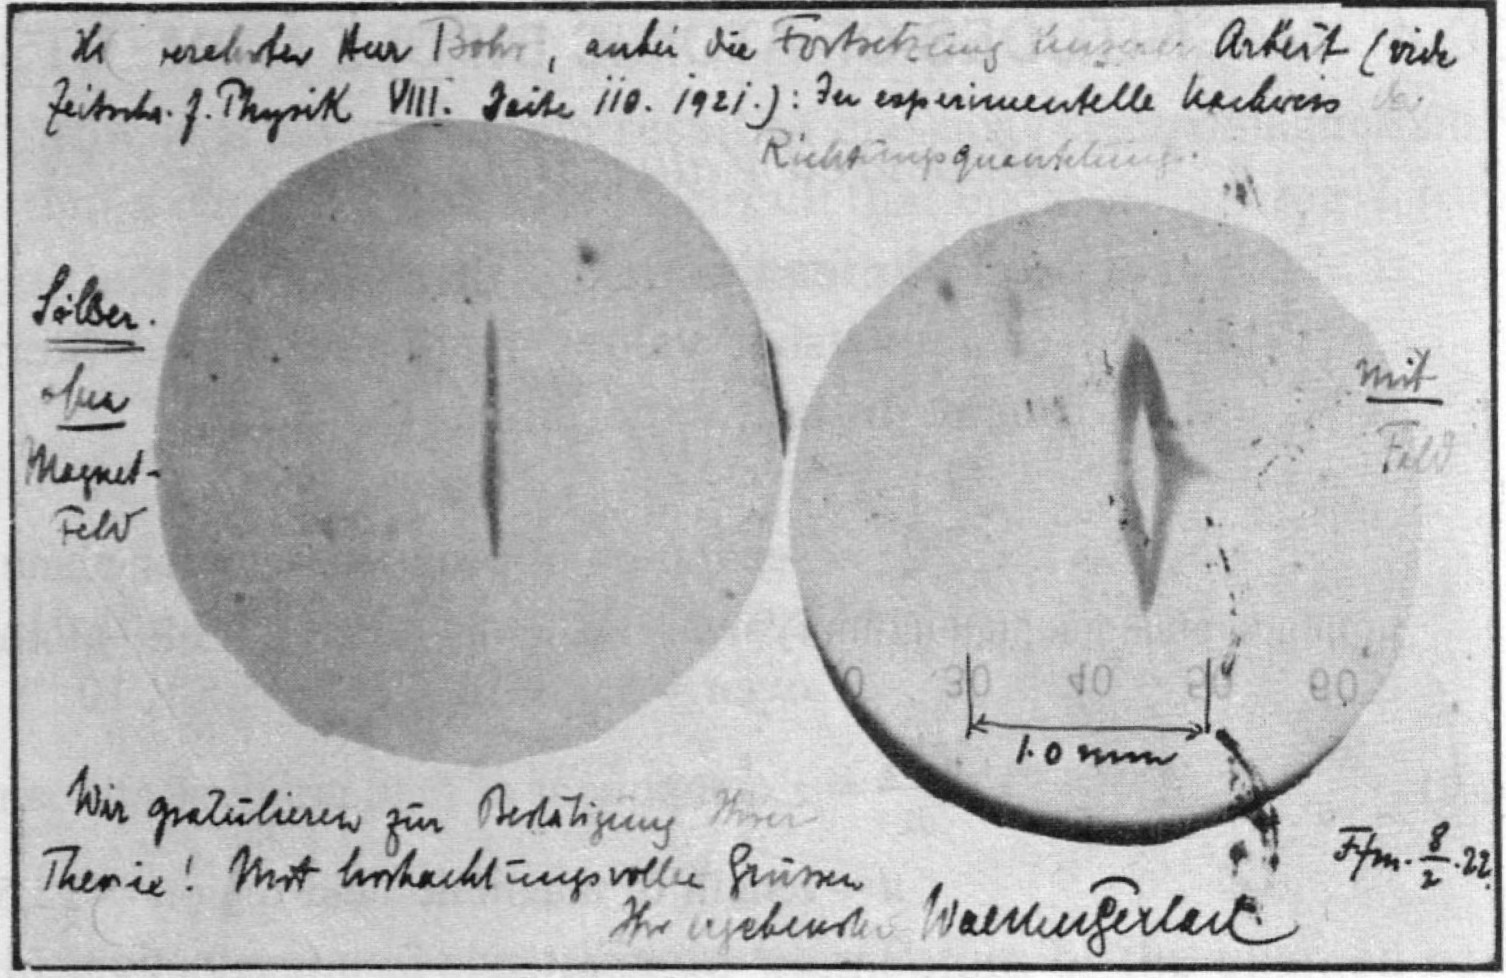
\includegraphics[width=10cm]{SGExperiment/sg-result.jpg}
\caption{斯特恩-盖拉赫实验的原始结果}
%\label{default}
\end{center}
\end{figure}

\subsection{连续的斯特恩-盖拉赫实验}

对我们的物理世界,选哪个方向是$z$方向是任意的,可以设想同样的实验对$x$或$y$取向的非均匀磁场也同样成立,即对$x$方向的非均匀磁场,我们会发现银原子会分裂为$x$正向和负向相同比例的两束,对应的就是自旋角动量在$x$方向上取$s_x = \pm \frac{1}{2} \hbar$的两类银原子。

真正有意思的是连续的斯特恩盖-拉赫实验\index{Stern-Gerlach experiment:斯特恩盖-拉赫实验},比如:我们可以让一束银原子通过$z$方向非均匀的磁场(记作SGz),得到在$z$方向分裂的两束,比如我们遮挡上其中一束,比如$s_z = - \frac{1}{2} \hbar$($s_z -$),我们让$s_z = \frac{1}{2} \hbar$的那一束($s_z +$)再次通过SGz装置,我们会发现从第二个SGz中出射的就只有$s_z +$的部分了。

这说明$s_z = \pm \frac{1}{2} \hbar$是互相排斥的两类,其分类标准由SGz装置定义,同时在此分类标准下分为两类又是个完全的分类(因为银原子只分裂为两束)。

我们可以让$s_z +$的成分继续通过一个$x$方向的非均匀磁场(SGx装置),此时发现银原子仍会分裂为延$x$方向正、负各50\%的两束。

这个结果是容易被人们接受的,这就相当于我们用不同于SGz所定义的分类标准对$s_z +$的成分进行第二轮筛选,其结果是分为$s_x = \pm \frac{1}{2} \hbar$($s_x \pm$)两类。

我们可以把$s_x -$的成分遮挡住,只引出$s_x +$的成分,使之再次通过$z$方向的非均匀磁场(SGz),现在的问题是银原子是会分裂为$s_z \pm$两束,还是只有$s_z +$一束?

\begin{figure}[htbp]
\begin{center}
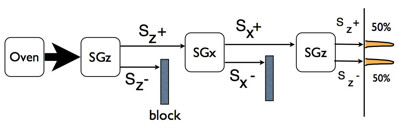
\includegraphics[width=10cm]{SGExperiment/SequentialSGE.jpg}
\caption{连续的斯特恩-盖拉赫实验}
%\label{default}
\end{center}
\end{figure}

直觉上我们会觉得只会得到$s_z +$一束,但实验结果却是仍然分裂为$s_z \pm$两束。这里我们选择充分相信实验的结果,不去质疑实验的设计与细节,在此前提下我们应如何理解这个结果呢?

从分类的角度,这里涉及两个不同分类标准,一个是$SGz$,一个是$SGx$,第一次筛选,我们只筛选出$s_z +$的成分,然后我们继续分类,换之以$SGx$标准,得到$s_x \pm$两类,但问题是在我们进行第二次分类的时候,银原子是否能够继续保持$s_z +$这一状态呢?

在量子力学I中,我们会说由于算符$s_z$和$s_x$是不对易的,因此不存在$s_z$和$s_x$同时取确定值的量子态(自旋量子数$s=0$的情形除外)。即如果我们知道银原子处在比如$s_x +$的状态,它就不可能同时处于$s_z +$的状态了。这说明理解斯特恩-盖拉赫实验对理解量子力学很重要。

理解新事情总是通过将其比拟为另一个(更熟悉的)事情来达成。比如连续的斯特恩-盖拉赫实验之所以难理解,是因为我们会把$s_z$和$s_x$想象为一个向量的在不同方向上的投影,这样$s_z$和$s_x$同时取确定值就是好理解的,而无法同时取确定值就是无法理解的。

\subsection{光学类比}

通过光学类比我们可以获得这种理解。

光波是电磁波,电磁波是横波,电场分量$\vec E$和磁场分量$\vec B$振荡的方向与电磁波传播的方向$\vec k$垂直。这样对电磁波而言就有了偏振\index{Polarized light:偏振光}的概念。

求解电磁波方程,会得到这样的关系\footnote{Electromagnetic radiation, \url{http://en.wikipedia.org/wiki/Electromagnetic_radiation};D. J. Griffiths, Introduction to Electrodynamics, pp379.},

\begin{equation}
\vec B = \frac{1}{c} \vec k \times \vec E 
\end{equation}

这里$c$是真空中得光速,这意味着对电磁波而言,我们只需考虑电场分量$\vec E$就够了。

x-偏振光:

\begin{equation}
\vec E_x = E_0 \hat x \cos (k z - \omega t )
\end{equation}

y-偏振光:

\begin{equation}
\vec E_y = E_0 \hat y \cos (k z - \omega t )
\end{equation}

偏振片能吸收特定方向振荡的电磁波,比如x-偏振片能吸收所有垂直于$x$方向的电场的能量,而让平行于$x$方向的电场的振荡穿透过去。我们可以通过旋转偏振片的方向使透射的光具有特定的偏振方向。

比如我们可以让x-偏振片逆时针旋转$45^o$得到x'-偏振光,继续旋转$90^o$得到y'-偏振光。

\begin{eqnarray}
\vec E_{x'} & = & \frac{E_0}{\sqrt 2} (\hat x + \hat y)  \cos (k z - \omega t ) \\
\vec E_{y'} & = & \frac{E_0}{\sqrt 2} ( - \hat x + \hat y)  \cos (k z - \omega t )
\end{eqnarray}

x/y-偏振光和x'/y'偏振光是对电磁波的两种不同分类方式,它们分别都是既不遗漏也不重复的分类方式。即x-偏振光中没有丝毫y-偏振光的成分,y-偏振光中也没有丝毫的x-偏振光的成分。

我们现在可以构造一个连续的偏振片的实验来类比连续的斯特恩-盖拉赫实验:首先让一束自然光通过x-偏振片,得到x-偏振光(对应$s_z +$),然后继续通过x'-偏振片,得到x'-偏振光(对应$s_x +$),最后使之通过y-偏振片。最终会有y-偏振光(对应$s_z -$)射出吗?

答案是肯定的,并且很容易理解,对x-偏振光而言,电场振荡的方向在$x$方向上,x-偏振光穿过x'-偏振片意味着垂直于$x'$方向的光会被吸收,而平行于$x'$方向的光会穿透出来,电场强度应是$\vec E_x$向$x'$方向做投影,因子为$\frac{1}{\sqrt 2}$,由于光强正比于电场强度的平方,因此正好有50\%的光会穿透过来。

现在,穿过x'-偏振片光的电场就在$x'$方向上了,再继续穿过y-偏振片,就是向$y$方向做投影,这样会再次得到因子$\frac{1}{\sqrt 2}$,...

这样我们就可以对银原子的量子态(即自旋1/2的量子态)建立起一个数学表示,我们用一个二维的列向量来表示自旋1/2的量子态,$s_z +$的态对应x-偏振光,我们把它表示为:

\begin{equation}
\left| s_z + \right\rangle = \left| + \right\rangle = \left( \begin{array}{cc} 1 \\ 0 \end{array} \right)
\end{equation}

类似地,用y-偏振光对应的二维列向量来表示$s_z -$的态:

\begin{equation}
\left| s_z - \right\rangle = \left| - \right\rangle = \left( \begin{array}{cc} 0 \\ 1 \end{array} \right)
\end{equation}

用x'-偏振光对应的二维列向量来表示$s_x +$的态:

\begin{equation}
\left| s_x + \right\rangle  = \frac{1}{\sqrt 2} \left( \begin{array}{cc} 1 \\ 1 \end{array} \right)
\end{equation}

用y'-偏振光对应的二维列向量来表示$s_x -$的态:

\begin{equation}
\left| s_x - \right\rangle  = \frac{1}{\sqrt 2} \left( \begin{array}{cc} -1 \\ 1 \end{array} \right)
\end{equation}

最后还剩两个态$s_y \pm$,我们用圆偏振光(右旋和左旋)对应的二维列向量来表示:

\begin{equation}
\left| s_y \pm \right\rangle = \frac{1}{\sqrt 2} \left( \begin{array}{cc} 1 \\ \pm i \end{array} \right)
\end{equation}

这意味着我们可用二维复系数线性向量空间中的一个向量来表示一个自旋1/2的量子态。

\subsection*{参考}

J. J. Sakurai, Modern Quantum Mechanics, \S 1.1

\section{平移算符}

\subsection{无穷小平移算符}

我们把无穷小平移\index{infinitesimal translation:无穷小平移}(infinitesimal translation)$T(dx')$定义为:

\begin{equation}
T(dx') \left| x' \right\rangle = \left| x' + dx' \right\rangle 
\end{equation}

效果上就是把位于$x'$附近的量子态平移到$x'+ dx'$位置附近。

根据物理上我们对空间的直觉,我们规定$T$应满足如下性质:

(1)幺正性:

平移不改变粒子数:$\left\langle \alpha | \alpha \right\rangle = \left\langle \alpha \right| T^\dagger T \left| \alpha \right\rangle  $,即要求:

\begin{equation}
T^\dagger (dx') T (dx') = 1
\end{equation}

(2)对连续的平移操作满足:

\begin{equation}
T( dx'' ) T (dx') = T(dx'' + dx')
\end{equation}

(3)逆操作就是反方向平移:

\begin{equation}
T^{-1} (dx') = T(- d x')
\end{equation}

(4)连续性:

\begin{equation}
\lim\limits_{dx' \to 0} T(dx') = 1
\end{equation}

可以证明,假如$T(dx')$取如下形式,

\begin{equation}
T(dx' ) = 1 - i K \cdot dx'
\end{equation}

并且算符$K$是厄米的($K^\dagger = K$),以上四条性质将自动满足。

由于$K$是厄米算符,根据量子力学它可对应某个力学量,其量纲为$\frac{1}{[ Length ]}$。

物理学首先在人的日常经验中被研究,所以最初的单位制是适合于人本身的尺度的,比如长度是米,时间是秒,质量是千克。而量子力学对应的是原子尺寸的物理现象,这样就涉及到一个换算的问题。$K$常被写为$\frac{p}{\hbar}$,这里$\hbar$是普朗克常数,量纲为$[Energy] [Time]$,$\hbar$很小,就是因为日常世界和量子世界尺度的不同引入的换算因子,因为如果我们首先发展的是量子力学我们本可以取$\hbar = 1$的。

现在$p$就对应某个力学量,其量纲为$\frac{[E] [T]}{[L]} = [M] \frac{[L]}{[T]}$,即动量的量纲。这样我们就把动量算符\index{momentum operator:动量算符}定义为无穷小平移算符的产生算符。

\begin{equation}
T(dx') = 1 - i \frac{p \cdot dx'}{ \hbar }
\end{equation}

\subsection{基础对易式}

我们可由无穷小平移算符$T(dx')$的表达式出发推出基础对易式\index{fundamental commutation relation:基础对易式}$[x, p_x] = i \hbar$。

首先计算对易式$[x, T(dx')]$,

\begin{eqnarray*}
x T (dx') \left| x' \right\rangle & = & (x' + dx' ) \left| x'+ dx' \right\rangle \\
T(dx' ) x \left| x' \right\rangle & = & x' T(dx') \left| x' \right\rangle = x' \left| x' + dx' \right\rangle
\end{eqnarray*}

由于$dx' \to 0$,以下计算只需要考虑$dx'$的一阶小量即可。得到,

\begin{equation}
[x, T(dx')] = dx'
\end{equation}

将上式展开:

\begin{equation}
- i x K \cdot dx' + i K \cdot dx' x = dx'
\end{equation}

需要注意的是以上$x$,$K$和$dx'$均是矢量(算符)。

假设$d \vec x'$在第1个方向上,即:$d \vec x' = d \vec x' \hat x_1 $,$\vec K \cdot d \vec x' = K_1 dx'$。

\begin{eqnarray*}
x_1 K_1 - K_1 x_1 & = & i \\
x_2 K_1 - K_1 x_2 & = & 0 \\
x_3 K_1 - K_1 x_3 & = & 0
\end{eqnarray*}

我们还可以取$d \vec x'$在第2个方向或第3个方向上。这样我们就得到:

\begin{equation}
[x_i , K_j ] = i \delta_{ij}
\end{equation}

$i$,$j$分别都可取1,2,3对应三维物理空间。我们还可把上式改写为以下常见的形式:

\begin{equation}
[x_i , p_j ] = i \hbar \delta_{ij}
\end{equation}

即基础对易式\index{fundamental commutation relation:基础对易式}(fundamental commutation relations)。

\subsection{动量算符}

由无穷小平移算符出发,

\begin{eqnarray*}
\left( 1- \frac{i p \Delta x'}{\hbar}  \right) \left| \alpha \right\rangle & = & \int dx' T(\Delta x') \left| x' \right\rangle \left\langle x' | \alpha \right\rangle \\
 {} & = & \int dx' \left| x' + \Delta x' \right\rangle \left\langle x' | \alpha \right\rangle  \\
 {} & = & \int dx' \left| x' \right\rangle \left\langle x- \Delta x' | \alpha \right\rangle \\
 {} & = & \int dx' \left| x' \right\rangle \left( \left\langle x' | \alpha \right\rangle - \Delta x' \frac{\partial }{\partial x'}  \left\langle x' | \alpha \right\rangle \right)
\end{eqnarray*}

即,

\begin{equation}
p \left| \alpha \right\rangle = \int dx' \left| x' \right\rangle \left( \frac{\hbar}{i} \frac{\partial }{\partial x'} \left\langle x' | \alpha \right\rangle  \right)
\end{equation}

左乘$\left\langle x' \right|$,可得:

\begin{equation}
\left\langle x' \right| p \left| \alpha \right\rangle = \frac{\hbar}{i } \frac{\partial }{\partial x'} \left\langle x' | \alpha \right\rangle
\end{equation}

如果把$\left| \alpha \right\rangle$替换为$\left| x'' \right\rangle$,就得到动量算符\index{momentum operator:动量算符}在位置表象下的矩阵表示:

\begin{equation}
\left\langle x' \right| p \left| x'' \right\rangle = \frac{\hbar}{i } \frac{\partial }{\partial x'} \left\langle x' | x'' \right\rangle = \frac{\hbar}{i } \frac{\partial }{\partial x'} \delta(x' - x'')
\end{equation}

\subsection*{参考}

J. J. Sakurai, Modern Quantum Mechanics, \S 1.6


\section{时间演化}

\subsection{时间演化算符}

量子态$\alpha$,初始时刻$t_0$,记作$\left| \alpha, t_0 \right\rangle$,由此演化到$t$时刻($t > t_0$)的量子态记作$\left| \alpha, t_0; t \right\rangle$。

定义演化算符$U(t, t_0)$,把初始态和由$t_0$演化到$t$的态联系起来,

\begin{equation}
\left| \alpha, t_0; t \right\rangle = U(t, t_0) \left| \alpha, t_0 \right\rangle 
\end{equation}

这样的算符就叫时间演化算符。

由时空的物理直觉出发,我们规定$U$应当满足的性质:

(1)幺正性:初始时刻态矢量归一,则$t$时刻态矢量也要归一,即:

\begin{equation}
\left\langle \alpha, t_0 | \alpha, t_0 \right\rangle = \left\langle \alpha, t_0; t | \alpha, t_0; t \right\rangle = 1
\end{equation}

这意味着:

\begin{equation}
U^\dagger (t, t_0) U (t, t_0) = 1
\end{equation}

(2)合成性质:

\begin{equation}
U(t_2, t_0) = U(t_2, t_1) U (t_1, t_0)
\end{equation}

物理系统由时间$t_0$演化到$t_2$,必须要先经历$t_0$和$t_2$之间的$t_1$。

(3)连续性:对无穷小时间演化$U(t_0+ dt, t_0)$,

\begin{equation}
\lim\limits_{dt \to 0} U(t_0 + dt, t_0) = 1
\end{equation}

我们可以验证,只要我们取无穷小时间演化算符\index{Infinitesimal time-evolution operator:无穷小时间演化算符}为如下形式,

\begin{equation}
U(t_0+dt, t_0) = 1- i \Omega dt
\end{equation}

其中$\Omega$是厄米算符,$\Omega^\dagger = \Omega $,以上性质即可自动得到满足。

由于$\Omega$是厄米算符,$\Omega$可对应一力学量,其量纲为$\frac{1}{[Time]}$,即频率的量纲。类似前面在无穷小平移算符中所讨论过的,我们把$\Omega$改写为$\frac{H }{\hbar}$,$\hbar$是作用量(action)量纲$[Energy] [Time]$,那么$H$就是能量量纲,即哈密顿算符。这样,

\begin{equation}
U(dt ) = 1- \frac{i H dt}{\hbar}
\end{equation}

\subsection{薛定谔方程}

由无穷小演化算符出发,我们可以推出薛定谔运动方程\index{Schr\"{o}dinger equation:薛定谔方程}(S.E.),首先由演化算符的合成性质:

\begin{equation*}
U(t+dt, t_0) = U(t+ dt , t) U(t, t_0) = \left( 1- \frac{i H dt}{\hbar}  \right) U(t, t_0)
\end{equation*}

调整一下等式左右两边的项:

\begin{equation*}
U(t+dt, t_0) - U(t, t_0) = -  i\frac{H}{\hbar} dt U(t, t_0)
\end{equation*}

就可得到演化算符$U$所满足的微分方程:

\begin{equation}
i \hbar \frac{\partial U(t, t_0) }{\partial t} = H U(t, t_0)
\end{equation}

右乘初始时刻态矢量$\left| \alpha, t_0 \right\rangle$,

\begin{equation}
i \hbar \frac{\partial }{\partial t} \left| \alpha, t_0; t \right\rangle  = H \left| \alpha, t_0; t \right\rangle
\end{equation}

这就是通常所说的薛定谔方程。

\subsection*{参考}

J. J. Sakurai, Modern Quantum Mechanics, \S 2.1

%%%%\input{TimeEvolution/CoherentState.tex}

\section{传播子}

\subsection{绘景回顾}

薛定谔绘景(S.P.)下,态矢量$\left| \alpha, t \right\rangle$含时,力学量不含时,态矢量随时间的演化符合薛定谔方程\index{Schr\"{o}dinger equation:薛定谔方程}。

\begin{equation}
i \hbar \frac{\partial }{\partial t} \left| \alpha, t \right\rangle = H \left| \alpha, t \right\rangle 
\end{equation}

其解可表示为:

\begin{equation}
\left| \alpha, t \right\rangle = U(t) \left| \alpha \right\rangle
\end{equation}

这里:

\begin{equation}
U(t) = e^{-iHt / \hbar}
\end{equation}

力学量$A$的本征值问题,

\begin{equation}
A \left| a' \right\rangle = a' \left| a' \right\rangle 
\end{equation}

定义了基矢(basis)$\left| a' \right\rangle$,$\left| a' \right\rangle$也不含时。

态矢量$\left| \alpha, t \right\rangle$含时,可以用基矢$\left| a' \right\rangle$展开:

\begin{equation}
\left| \alpha, t \right\rangle = \sum\limits_{a'} \left| a' \right\rangle \left\langle a' | \alpha, t \right\rangle 
\end{equation}

这里含时的部分被包含在因子$\left\langle a' | \alpha, t \right\rangle $中。

对海森堡绘景(H.P.)而言,态矢量不含时,比如就取$t=0$时刻时候的态矢量,记作:$\left| \alpha \right\rangle$。力学量含时,

\begin{equation}
A(t) = U^\dagger (t) A U (t)
\end{equation}

符合海森堡运动方程,

\begin{equation}
i \hbar \dot A = [A, H]
\end{equation}

现在来考虑H.P.下力学量$A(t)$的本征值问题:

\begin{equation}
A(t) \left| a', t \right\rangle = a' \left| a', t \right\rangle
\end{equation}

考虑到,

\begin{equation}
U^\dagger A U U^\dagger \left| a' \right\rangle = a' U^\dagger \left| a' \right\rangle
\end{equation}

H.P.下的基矢是:

\begin{equation}
\left| a', t \right\rangle = U^\dagger \left| a' \right\rangle
\end{equation}

看起来和S.P.下态矢量$\left| \alpha , t \right\rangle$随时间的演化$\left| \alpha , t \right\rangle = U \left| \alpha \right\rangle$类似,但方向正好相反。

\subsection{传播子}

在S.P.下,给定量子系统$H = \frac{p^2}{2m} + V$,考虑态矢量由$\left| \alpha , t_0 \right\rangle$演化到$\left| \alpha , t \right\rangle$,

\begin{equation}
\left| \alpha , t \right\rangle = e^{-i H (t - t_0) / \hbar}  \left| \alpha , t_0 \right\rangle
\end{equation}

考虑$[A, H ] = 0$,基矢$\left| a' \right\rangle$同时也是$H$的本征矢,$H \left| a' \right\rangle = E_{a'} \left| a' \right\rangle $,因此:

\begin{equation}
\left| \alpha , t \right\rangle = \sum\limits_{a'} \left| a' \right\rangle \left\langle a' | \alpha, t_0 \right\rangle e^{-i E_{a'} (t - t_0) / \hbar}
\end{equation}

左乘$\left\langle x' \right|$,把上式变到位置表象,

\begin{equation}
\left\langle x' | \alpha, t \right\rangle = \sum\limits_{a'} \left\langle x' | a' \right\rangle \left\langle a' | \alpha, t_0 \right\rangle e^{- i E_{a'} (t - t_0) / \hbar}  
\end{equation}

把因子$\left\langle a' | \alpha, t_0 \right\rangle$表示为位置表象,

\begin{equation}
\left\langle a' | \alpha, t_0 \right\rangle = \int d^3 x \left\langle a' | x' \right\rangle \left\langle x' | \alpha, t_0 \right\rangle 
\end{equation}

为了避免歧义,把$\left\langle x' | \alpha, t \right\rangle$中的$x'$改记为$x''$,

\begin{equation}
\left\langle x'' | \alpha, t \right\rangle = \int d^3 x' \sum\limits_{a'}  \left\langle x'' | a' \right\rangle \left\langle a' | x' \right\rangle e^{- i E_{a'} (t - t_0) / \hbar} \left\langle x' | \alpha, t_0 \right\rangle
\end{equation}

定义积分的核(Kernel)为$K(x'', t; x', t_0)$,

\begin{equation}
K(x'', t; x', t_0) = \sum\limits_{a'}  \left\langle x'' | a' \right\rangle \left\langle a' | x' \right\rangle e^{- i E_{a'} (t - t_0) / \hbar}
\end{equation}

并用波动力学中的波函数对上上式进行改写,

\begin{equation}
\psi_\alpha (x'', t ) = \int d^3 x' K(x'', t; x', t_0) \psi_\alpha (x', t_0 )
\end{equation}

我们称$K$为传播子\index{Propagator:传播子},即描述由时空中$x', t_0$传播到$x'', t$的行为。传播子与初始时刻的波函数$\psi_\alpha (x', t_0 )$无关,它是物理系统($H$,这里就是$V$)本身性质的反映。

只要知道$\psi_\alpha (x', t_0 )$和$K$,就可知道$t > t_0$时刻的波函数$\psi_\alpha (x'', t )$。即是决定的,是因果律的。

\begin{equation*}
i \xrightarrow{K}{} f
\end{equation*}

\subsection{传播子的性质}

(1)对$t > t_0$,传播子$K$符合薛定谔方程(S.E.)

(2)当$t \to t_0$时,传播子是德尔塔函数,

\begin{equation}
\lim\limits_{t \to t_0} K = \lim\limits_{t \to t_0} \sum\limits_{a'} \left\langle x'' | a' \right\rangle \left\langle a' | x' \right\rangle e^{- i E_a' (t - t_0) / \hbar} = \left\langle x'' | x' \right\rangle
\end{equation}

(3)$K$可表示为:

\begin{equation}
K = \left\langle x'' \right| e^{- i H (t - t_0) / \hbar}  \left| x' \right\rangle  
\end{equation}

证明:

\begin{equation*}
K = \sum\limits_{a'} \left\langle x'' \right| e^{- i H (t - t_0) / \hbar} \left| a' \right\rangle \left\langle a' | x' \right\rangle = ...  
\end{equation*}

(4)$K$是格林函数(G.F.)

与电动力学中给定电荷分布求电动势类比,

\begin{equation}
\phi(x) = \int d^3 x' \frac{\rho (x')}{ \left| x - x' \right| }
\end{equation}

这里$\phi(x)$和$\psi_\alpha (x'', t)$对应,$\rho(x')$和$\psi_\alpha (x', t_0)$对应,而$\frac{1}{ \left| x - x' \right| }$和传播子$K$对应,都是积分的核。

$\frac{1}{ \left| x - x' \right| }$是微分方程$\nabla \cdot \nabla \frac{1}{ \left| x - x' \right| }  = \delta^3 (x- x')$的解,类似地$K$是如下方程的解,

\begin{equation}
\left[ i \hbar \frac{\partial }{\partial t} + \frac{\hbar^2}{ 2m} \nabla''^2 - V(x'')  \right] K = i \hbar \delta^3 (x'' - x') \delta (t - t_0)
\end{equation}

即:

\begin{equation}
\left[ i \hbar \frac{\partial }{\partial t} - H \right] K = i \hbar \delta^3 (x'' - x') \delta (t - t_0) 
\end{equation}

边条件是$t < t_0$时,$K = 0$。对应推迟解,或符合因果律的解(时间在前的影响时间在后的,而非相反)。

$K$就是数学上的格林函数\index{Green Function:格林函数}(Green Function,G.F.),其定义为微分算子作用于格林函数等于德尔塔函数,即$\hat L G(x,s) = \delta(x-s)$。

\subsection{态的求和}

考虑$x'' = x'$,$t_0 = 0$,则$K (x', t ; x', 0)$

定义格林函数为:

\begin{equation}
G(t) = \int d^3 x' K(x', t; x', 0) = ... = \sum\limits_{a'} e^{-i E_{a'} t / \hbar}
\end{equation}

如此定义的G.F.,就等于对所有量子态$a'$的求和(sum over states)。

我们可以把$G(t)$与统计力学中的配分函数\index{partition function:配分函数}(partition function,Z)进行比较,

\begin{equation}
Z = \sum\limits_{a'} e^{- \beta E_{a'}}
\end{equation}

这两个式子都是对所有量子态$a'$的求和。

引入虚时变换,

\begin{equation}
\beta = \frac{i t }{\hbar }
\end{equation}

这两个求和在数学上有相同的形式,这意味着我们在量子力学(量子场论)中发展出来的方法可以直接应用于量子统计。

$G(t)$的宗量是时间,为了更方便地考察其中的物理,我们往往把时间宗量$t$变为能量宗量$E$(或频率宗量$\omega$,考虑到$E = \hbar \omega$,这其实是一回事)。

\begin{equation}
\widetilde{G} (E) = - \frac{i}{\hbar } \int_0^{\infty} dt G(t ) e^{i Et / \hbar}
\end{equation}

但这样积分积出来是不定的(存在$e^{i \infty}$的项),为了避免这个困难,我们把$E$拓展到复平面,并考虑变量变换$E \to E + i 0^+$,这样我们就得到,

\begin{equation}
\widetilde{G} (E) = \sum\limits_{a'} \frac{1}{ E - E_{a'}}
\end{equation}

这意味着我们只需研究格林函数$\widetilde{G} (E)$在复$E$平面的解析性质(奇点位置)就可知道给定物理系统的能谱$\{ E_{a'} \}$。

\subsection{海森堡绘景下的传播子}

传播子$K (x'',t; x',t_0) = \left\langle x'' \right| e^{- i H (t - t_0) / \hbar} \left| x' \right\rangle$是在薛定谔绘景(S.P.)下的定义。

在海森堡绘景\index{Heisenberg Picture:海森堡绘景}下,利用$\left| a' , t \right\rangle = U^\dagger \left| a' \right\rangle$

\begin{equation}
K = \left\langle x'' \right| U(t) U^\dagger (t_0 ) \left| x' \right\rangle = \left\langle x'', t | x', t_0 \right\rangle
\end{equation}

传播子$K$即变换幅\index{Transition amplitude:变换幅}(Transition amplitude),$\left\langle x'', t | x', t_0 \right\rangle$的含义是“粒子”由$x', t_0$出发,传播到$x'', t$处的几率幅。

\subsection*{参考}

J. J. Sakurai, Modern Quantum Mechanics, \S 2.2 \S 2.5

\section{路径积分}

\subsection{变换幅}

H.P.下,传播子$K(x,t;x_0,t_0)$可写为初始时刻位置算符本征矢$\left| x_0, t_0 \right\rangle$与终了时刻位置算符本征矢$\left| x,t \right\rangle$的内积。$\left| x_0, t_0 \right\rangle$与$\left| x, t \right\rangle$分别都可构成表示量子态的基矢量。传播子\index{Propagator:传播子}的地位就相当于由初始时刻(A)到终了时刻(B)的表象变换,

\begin{equation}
K(xt; x_0,t_0) = \left\langle x,t | x_0, t_0 \right\rangle
\end{equation}

就相当于是AB表象之间的变换矩阵,现在因为位置的取值是连续的,我们可以管$\left\langle x,t | x_0, t_0 \right\rangle$叫变换函数(transformation function),它把不同时刻($t$和$t_0$)的两套基矢联系起来。

$t> t_0$,在$t$与$t_0$之间我们总可插入一个时刻$t_1$,量子态由$t_0$开始,先演化到$t_1$,最后演化到终了时刻$t$,这相当于我们在变换幅$\left\langle x,t | x_0, t_0 \right\rangle$中间插入一个单位算符:

\begin{equation}
1 = \int d^3 x_1 \left| x_1, t_1 \right\rangle \left\langle x_1, t_2 \right|
\end{equation}

这里$\left| x_1, t_1 \right\rangle$是$t_1$时刻,位置算符的本征矢,它的集合也构成一个基矢。现在变换幅表示为:

\begin{equation}
\left\langle x,t | x_0, t_0 \right\rangle = \int d^3 x_1 \left\langle x,t | x_1, t_1 \right\rangle \left\langle x_1 , t_1 | x_0, t_0 \right\rangle
\end{equation}

上式称为变换幅的合成性质(composition property),利用这一性质我们可以继续插入不同时刻的位置算符的本征矢,直至相邻时间间隔$d t \to 0$为止。当$d t \to 0$时,变换幅将有可能表现为简单的形式,循此思路,费曼提出了量子力学的路径积分表示,这是不同于波动力学和矩阵力学的第三种量子力学的表述方式。

\subsection{路径求和}

假设我们在$t_0$到$t$区间里插入$N$个时刻,$t_1, t_2, ..., t_N$,当$N \to \infty$时,每相邻时间间隔$\frac{t - t_0}{N} \to 0$。

现在,$x_0,t_0$到$x,t$的变换幅可表示为:

\begin{equation}
\left\langle x,t | x_0, t_0 \right\rangle = \int d^3 x_N ... \int d^3 x_1 \left\langle x, t | x_N, t_N \right\rangle \left\langle  ... \right\rangle ... \left\langle x_1, t_1 | x_0 , t_0 \right\rangle
\end{equation}

积分就是求和,被求和的项是:

\begin{equation*}
\left\langle x,t | N \right\rangle \left\langle N | N-1 \right\rangle ... \left\langle 2 | 1 \right\rangle \left\langle 1 | 0 \right\rangle
\end{equation*}

共$N+1$个无穷小时间间隔的传播子相乘,如果我们追踪每个时间的节点的话,首先由$t_0$出发,$0 \to 1$是第一个传播子,0点作为初始点是固定的,但1点作为积分中的哑元需遍历全空间,假如追踪某个特定的1点,将继续传播到2,$1 \to 2$,同样2点也需遍历全空间,……,最后由N点回到终了时刻$t$。

从$t_0$到$t$构成了一个互相连接的传播子路径,但这个路径中只有首、尾两点是固定的,中间N个节点可以有多种选择,并且需遍历整个空间。这样总的传播子(或变换幅)$\left\langle x,t | x_0, t_0 \right\rangle$就相当于是首尾固定情况下所有“各种路径”的求和。

\begin{equation}
\left\langle x,t | x_0, t_0 \right\rangle \propto \sum\limits_{All Paths} \left\langle x, t | x_N, t_N \right\rangle \left\langle  ... \right\rangle ... \left\langle x_1, t_1 | x_0 , t_0 \right\rangle   
\end{equation}

量子力学中真正关键的是相位,现在每一个无穷小传播子都带着一个相位,所有这些相位要加起来才对应某条路径的相位,不同路径的相位还会发生“干涉”,正是这个缘由导致了不同于经典物理的(丰富的)量子行为。

经典物理中涉及路径的基本原理有光程取极值原理(光学中的费马原理\index{Fermat's principle:费马原理})和力学中的最小作用量原理\index{Principle of least action:最小作用量原理}(哈密顿原理)。

前者是说光实际走过的路径是使光程取极值的路径,表示成数学形式就是:

\begin{equation}
\delta \int n(x) dx = 0 
\end{equation}

后者是说对经典力学而言,粒子实际走过的路径是使作用量取极值的路径,即:

\begin{equation}
\delta \int_{t_1}^{t_2} L_c (x, \dot x) dt = 0
\end{equation}

由费马原理可解释光的直线传播,反射、折射定律等。由哈密顿原理,我们可求出粒子运动的动力学方程:

\begin{equation}
\frac{d}{dt } \frac{\partial L_c}{\partial \dot x} - \frac{\partial L_c }{\partial x} = 0
\end{equation}

上式其实就是:$m \ddot x =  - \frac{\partial V}{ \partial x}$

既然通过(和路径相关的)作用量取极值的方法可以建立经典力学,那么我们是否可类似地基于路径和作用量的概念建立量子力学呢?这个思路对物理学家来说并不陌生,比如量子力学的对易式就可与经典力学中的泊松括号类比。

尽管如此量子力学和经典力学的结果还是有很大区别的,比如经典力学求出来的是一条确定的轨迹,而量子力学中的“对各种路径”求和,则表明每一条路径(而非只有某个特殊的路径)都会对最终的变换幅有贡献。我们期待当$\hbar \to 0$时,量子力学的结果会无限趋近经典力学的结果。

\begin{equation*}
Q.M. \xrightarrow{\hbar \to 0} C.M.
\end{equation*}

\subsection{费曼的路径积分}

量子力学的路径积分表示是由费曼完成的,费曼研究生的时候在狄拉克的书里读到:传播子$\left\langle x_2, t_2 | x_1, t_1 \right\rangle$就相当于(correspons to)是:

\begin{equation}
\exp \left[ {\frac{i \int_{t_1}^{t_2} L_c(x, \dot x) dt}{\hbar}} \right]
\end{equation}

积分部分是作用量(Action)$S$,其量纲与普朗克常数$\hbar$相同。$e$指数部分的$ \frac{i S(2,1)}{\hbar}$给定了传播子$\left\langle x_2, t_2 | x_1, t_1 \right\rangle$的相位。但传播子的振幅是什么,狄拉克并没有继续讨论。费曼读到这段后,深感困惑,他想弄明白这个“相当于”指的到底是什么,是“等于”,还是“正比于”,还是别的什么关系……经过计算,费曼发现这个“相当于”是“正比于”的意思,并求出了比例因子。

$\hbar$处于分母位置还能解释为什么当$\hbar \to 0$时,量子行为会过渡到经典行为。量子行为对应的是所有路径求和,而经典路径对应的是只有最小作用量的路径会凸显出来。最小作用量的路径就是使$\delta S = 0$的路径,在这个路径的附近还有很多其它路径,这些路径与最小作用量路径的偏离就是$\delta S$,而$\hbar $是趋于0的,但并不是0,在这个条件下,最小作用量附近路径的相位就是$e^{\frac{i \delta S}{ \hbar}}$,都趋于1,即相长干涉,因此经典路径的贡献就会加强凸显出来。

对一般的路径 $ \delta S \neq 0$,这意味着它和它附近路径的相位差是$\frac {\delta S} { \hbar } $,这里$ \delta S \neq 0 $,而$\hbar \to 0 $,$\frac{\delta S}{\hbar} $ 就是个很大的不确定的数,反映在相位上就是任意相位,这样对一般路径而言,它附近的那些路径与它的相位差是任意取值的,因此会互相抵消掉。这样在 $\hbar \to 0$ 时,那些非经典路径的变换幅就只能取0了。

%当然费曼最感困惑的是为什么狄拉克自己没有继续这个思路,进而提出量子力学的路径积分表示。据说他曾经就此问过狄拉克,但狄拉克没有告诉他。

现在我们来计算某个无穷小的传播子:

\begin{equation}
\left\langle x_n, t_n | x_{n-1}, t_{n-1} \right\rangle = \frac{1}{w(\Delta t)} e^{iS(n, n-1) / \hbar}
\end{equation}

这里$\Delta t = t_n - t_{n-1}$,$\frac{1}{w(\Delta t)}$是比例因子,假设它只和$\Delta t$有关。现在来计算$S(n, n-1)$,

\begin{equation}
S(n, n-1) = \int_{t_{n-1}}^{t_n} \left( \frac{m \dot x^2}{2}  - V(x) \right) dt
\end{equation}

由于$\Delta t \to 0$,我们可以把积分进行改写,

\begin{equation}
S(n, n-1) = \left[  \frac{m}{2} \left( \frac{x_n - x_{n-1} }{\Delta t} \right)^2 -V \left( \frac{x_n + x_{n-1}}{2} \right) \right] \Delta t
\end{equation}

假设我们研究的是自由粒子,$V=0$,现在无穷小的传播子变为:

\begin{equation}
\left\langle x_n, t_n | x_{n-1}, t_{n-1} \right\rangle = \frac{1}{w(\Delta t)} e^{ \frac{i m ( x_n - x_{n-1} )^2 }{ 2 \hbar \Delta t} }
\end{equation}

从样子上看,很像一个钟形函数(bell function,或高斯函数),$\Delta t$正比于钟形函数的宽度,当$\Delta t$趋于零时,钟形函数会变得无穷窄,即趋于一个德尔塔函数的样子。

当$\Delta t \to 0$时,即$t_n \to t_{n-1}$时,

\begin{equation}
\lim\limits_{t_n \to t_{n-1}} \left\langle x_n, t_n | x_{n-1}, t_{n-1} \right\rangle = \delta(x_n - x_{n-1}) 
\end{equation}

我们引入新的变量$\xi = x_n - x_{n-1}$,现在的问题就是当$\frac{1}{w(\Delta t)} =?$的时候,

\begin{equation}
\lim\limits_{\Delta t \to 0}  \frac{1}{w (\Delta t)} e^{\frac{i m \xi^2}{2 \hbar \Delta t}} = \delta (\xi) 
\end{equation}

考虑到德尔塔函数的性质,

\begin{equation}
\int \delta(\xi) d \xi =  \lim\limits_{\Delta t \to 0} \int d \xi  \frac{1}{w (\Delta t)} e^{\frac{i m \xi^2}{2 \hbar \Delta t}}   = 1 
\end{equation}

由高斯积分,

\begin{equation}
\int d \xi e^{\frac{i m \xi^2 }{ 2 \hbar \Delta t}  } = \sqrt{ \frac{ 2 \pi i \hbar \Delta t }{m } }
\end{equation}

我们就得到:

\begin{equation}
\frac{1}{w(\Delta t )} = \sqrt{\frac{m }{2 \pi i \hbar \Delta t} }
\end{equation}

最终我们就得到传播子的费曼路径积分\index{Path Integral:路径积分}表示:

\begin{equation}
\left\langle x_N,t_N | x_0, t_0 \right\rangle = \lim\limits_{N \to \infty} \left( \frac{m }{2 \pi i \hbar \Delta t } \right)^{N/2} \int dx_{N-1} ... \int dx_1 \prod\limits_{n=1}^{n = N} e^{\frac{iS(n, n-1)}{\hbar}} 
\end{equation}

我们可示意性地将其改写为:

\begin{equation}
\left\langle x_N,t_N | x_0, t_0 \right\rangle = \int_{x_0}^{x_N} D[x(t)] e^{ \frac{ i }{ \hbar} \int_{t_0}^{t_N} L_c(x, \dot x) dt }
\end{equation}

如此繁复的积分使得路径积分法在求解(非相对论)量子力学问题时没什么优势,但当使用路径积分求解量子场论(或多体)问题时却会变得很强大。

最后,我们还可验证如此求出的传播子$\left\langle x,t | x_0, t_0 \right\rangle$符合薛定谔方程(S.E.),即:

\begin{equation}
i \hbar \frac{\partial }{\partial t } \left\langle x,t | x_0, t_0 \right\rangle = - \frac{\hbar^2}{ 2 m } \frac{\partial^2 }{\partial x^2 } \left\langle x,t | x_0, t_0 \right\rangle + V (x) \left\langle x,t | x_0, t_0 \right\rangle
\end{equation}

\subsection*{参考}

J. J. Sakurai, Modern Quantum Mechanics, \S 2.5

R. P. Feynman, The Development of the Space-Time View of Quantum Electrodynamics.
\url{http://www.nobelprize.org/nobel_prizes/physics/laureates/1965/feynman-lecture.html}

\section{转动和角动量}

\subsection{三维实空间中的转动}

有限大小的物体可以在三维实空间中转动,这是人们的日常经验。现在假设我们研究的是刚体\index{Rigid body:刚体}(Rigid body),即物体的大小、形状及物体各部分与各部分之间的关系都是完全被规定而且是不变的情况。

任意的转动可以被描述为:(1)刚体围绕某个确定的转轴;(2)按右手螺旋转了一个角度。

这两个陈述要拿到一起来看,首先转轴的取向与刚体旋转的方向要构成一个“右手法则”,即右手大拇指的指向要指在转轴的取向上,与此同时右手的其它四个手指自然握紧的方向要与刚体旋转的方向一致。

在这样的约定下,我们需要三个参数来描述刚体的转动,首先转轴的取向需要两个参数,一个是转轴与$z$轴的夹角(polar angel),一个是转轴在$xy$平面上的方位角(azimuthal angel)。

刚体在三维实空间中的转动可以看做是我们施与刚体的一个操作,这个操作被记为$R_{\hat n}(\phi)$,这里单位向量$\hat n$表示转轴的取向,$\phi$表示刚体旋转的角度。

我们可以对刚体施与连续的操作$A$,$B$,这里$A$和$B$表示两个不同的转动,作为一个重要的经验,我们知道转动的后果,与我们实施转动的次序是有关的,用符号的语言表示就是$AB$未必与$BA$相同。

我们知道:如果是定轴转动,转动的效果与转动的次序无关,即$AB = BA$;但如果是定点转动,$A$和$B$两次转动的转轴不在一条直线上,那么$AB$的效果就与$BA$不同。

(这里我们约定转动的次序是从右到左依次进行的,即对依次进行的转动$AB$而言,我们先进行的是$B$操作,然后进行的是$A$操作。)

作为例子我们可以考虑转动$R_x(\frac{\pi}{2})R_z(\frac{\pi}{2})$和$R_z(\frac{\pi}{2})R_x(\frac{\pi}{2})$:

\begin{figure}[htbp]
\begin{center}
\includegraphics[width=9cm]{AngularMomentum/Rotation.png}
\caption{三维实空间中的转动}
%\label{default}
\end{center}
\end{figure}

如图我们用一个带红色箭头的矩形代表刚体,矩形的短边和长边可以区分前后、左右,而附带的红色箭头可用来表示上下。上半图表示的是$R_x(\frac{\pi}{2})R_z(\frac{\pi}{2})$,即先围绕$z$轴转$90^o$再围绕$x$轴转$90^o$,最终结果是红色的箭头向左。下半图是$R_z(\frac{\pi}{2})R_x(\frac{\pi}{2})$,最终的结果是红色箭头向前。即围绕不同转轴的转动操作与实施的次序有关。

对给定刚体,我们可以用某个向量$V$来表示刚体上的任意一点,在转动操作下,向量$V$会变换为$R V$,我们的日常经验告诉我们转动不会改变向量$V$的大小,

\begin{equation}
\left( R V \right)^T RV = V^T R^T R V = V^T V 
\end{equation}

这里$V$是个三维列向量,表示物理空间中的一个向量,$R$是个$3 \times 3$的正交矩阵\index{Orthogonal matrix:正交矩阵}(Orthogonal matrix),即:

\begin{equation}
R^T R = 1
\end{equation}

但其实光这个还不够,因为一般我们不把像空间反演\index{inversion:空间反演}(inversion)或照镜子这样的操作称为转动,比如我们会说在三维实空间中,无论你怎么转动都不能把你的左手转到和你的右手完全“重合”。所以我们还要附加一个条件,就是:

\begin{equation}
\det R = 1
\end{equation}

很容易验证,对空间反演矩阵$i = \left( \begin{array}{ccc} -1 & 0 & 0 \\ 0 & -1 & 0 \\ 0 & 0 & -1 \end{array} \right)$,或一个$x-y$平面上的“照镜子”$ m_{xy} = \left( \begin{array}{ccc} 1 & 0 & 0 \\ 0 & 1 & 0 \\ 0 & 0 & -1 \end{array} \right) $,有$\det i = -1$ 和 $ \det m_{xy} = -1$。

现在我们就可以用一个$\det R = 1$的三维正交矩阵来表示一个三维实空间中的转动。在群论的语言里,我们说这种对转动的表示构成了一个SO(3)群,3表示三维,O表示正交,而S表示“特殊”($\det R = 1$),一个“特殊的三维正交群”。

利用解析几何知识,我们很容易求出$R_z(\phi)$的形式:

\begin{equation}
R_z (\phi) = \left( \begin{array}{ccc} \cos \phi & - \sin \phi & 0 \\ \sin \phi & \cos \phi & 0 \\ 0 & 0 & 1 \end{array} \right)
\end{equation}

类似还可写出$R_x (\phi)$和$R_y (\phi)$(把矩阵中得行和列按规则的方式进行上下和左右的平移,并注意在此过程中保证$\det R = 1$)。

\begin{eqnarray}
R_x (\phi) & = & \left( \begin{array}{ccc} 1 & 0 & 0 \\ 0 & \cos \phi & - \sin \phi \\ 0 & \sin \phi & \cos \phi \end{array} \right) \\
R_y (\phi) & = & \left( \begin{array}{ccc} \cos \phi & 0 & \sin \phi \\ 0 & 1 & 0 \\ - \sin \phi & 0 & \cos \phi \end{array} \right)
\end{eqnarray}

我们特别关心无穷小的转动,这里我们取$\phi = \epsilon$,并对矩阵元进行展开,$\cos \epsilon$没有一阶无穷小,为了得到有意义的结果,我们展开到小量$\epsilon$的二阶。

\begin{equation}
R_z (\epsilon) = \left( \begin{array}{ccc} 1- \frac{\epsilon^2}{2} & - \epsilon & 0 \\ \epsilon & 1- \frac{ \epsilon^2 }{2} & 0 \\ 0 & 0 & 1 \end{array} \right)
\end{equation}

\begin{equation}
R_x (\epsilon) = \left( \begin{array}{ccc} 1 & 0 & 0 \\ 0 & 1- \frac{ \epsilon^2 }{2} & - \epsilon \\ 0 & \epsilon & 1 - \frac{\epsilon^2}{2} \end{array} \right)
\end{equation}

\begin{equation}
R_y (\epsilon) = \left( \begin{array}{ccc} 1- \frac{\epsilon^2}{2} & 0 & \epsilon \\ 0 & 1 & 0 \\  - \epsilon & 0 & 1 - \frac{\epsilon^2}{2} \end{array} \right)
\end{equation}

我们把$R_x(\epsilon)$,$R_y(\epsilon)$代入$R_x (\epsilon) R_y (\epsilon) - R_y (\epsilon) R_x (\epsilon) $中,得到:

\begin{equation*}
\left( \begin{array}{ccc}  0 & - \epsilon^2 & 0 \\  \epsilon^2 & 0 & 0 \\ 0 & 0 & 0 \end{array} \right)
\end{equation*}

即:

\begin{equation}
R_x (\epsilon) R_y (\epsilon) - R_y (\epsilon) R_x (\epsilon) = R_z ( \epsilon^2 ) - 1
\end{equation}

\subsection{对态矢量的无穷小转动}

上一小节我们讨论了对三维实空间中的转动,并得到了一个对转动的数学表示,即用一个行列式为1的三维正交矩阵去表示。这里的转动是针对三维真实物理向量$V$实施的,所谓刚体只不过是无穷多个关系固定的三维向量的集合(当然对每个向量还需附加一个质量密度)。

在量子力学中我们用一个态矢量$\left| \alpha \right\rangle$来描述物理系统的运动状态,态矢量不存在于真实的物理空间,它是数学空间(希尔伯特空间\index{Hilbert Space:希尔伯特空间})中的一个向量。而这个数学空间的维度与真实物理空间的维度是两回事,我们生活的物理世界是三维的,但对希尔伯特空间而言却可以是任意多维的(比如对自旋,我们就用一个二维复线性系数向量空间来描述态矢量)。

我们现在关心的是当物理系统在经历一个真实的转动(用$R$来表示)的同时,描述它的态矢量是如何随之变换的,我们认为会有一个希尔伯特空间中的变换算符($D(R)$)来联系其转动前($\left| \alpha \right\rangle$)和转动后($\left| \alpha \right\rangle_R$)的态矢量:

\begin{equation}
\left| \alpha \right\rangle_R = D(R) \left| \alpha \right\rangle
\end{equation}

这里$D$是德文转动一词“Drehung”的首字母。在三维实空间转动$R$的作用下:

\begin{eqnarray*}
V  &  \xrightarrow {R}  &   RV \\
\left| \alpha \right\rangle   &   \xrightarrow {R}  &  D(R)  \left| \alpha \right\rangle 
\end{eqnarray*}

类似于我们曾经对平移算符和时间演化算符的讨论,我们要求“转动”前的态矢量和“转动”后的态矢量“大小”不变,这要求转动算符$D(R)$是个幺正算符。模仿从前的思路,我们也讨论无穷小转动对应的$D(R)$,它将也被写为:

\begin{equation*}
1 - iG \epsilon
\end{equation*}

的形式,这里$G$是个厄米算符,因此有一个物理量与之对应,在经典物理中与转动对应的物理量是角动量\index{Angular Momentum:角动量}(Angular Momentum),于是我们也称这个物理量为角动量。

这样由旋转对称性的考虑出发,我们就得到了量子力学中角动量的定义,在这个定义中我们并没有用到经典物理中轨道角动量$\vec x \times \vec p$的定义形式,因此这个定义就超出了轨道角动量,把轨道和自旋角动量都放到同一个框架下来研究。

假设转轴的取向是$\hat n$,我们用$J \cdot {\hat n}$来表示延$\hat n$取向的角动量,由于单位选取的缘由,我们用$\frac{J \cdot {\hat n}}{\hbar} \to G$。

无穷小的对态矢量的转动就是:

\begin{equation}
D( R_{\hat n}( d \phi) ) = D (\hat n, \phi) = 1 - i \frac{ J \cdot \hat n}{ \hbar} d \phi
\end{equation}

比如,我们可以写出$D_x (d \phi)$等,

\begin{equation}
D_x(d \phi) = 1 - i \frac{J_x d \phi }{ \hbar }
\end{equation}

在上一小节中我们曾推出对无穷小三维实空间转动$R$存在以下关系:

\begin{equation*}
R_x (\epsilon) R_y (\epsilon) - R_y (\epsilon) R_x (\epsilon) = R_z ( \epsilon^2 ) - 1
\end{equation*}

现在$D(R)$也是对应$R$的,或者说$D(R)$也构成了对旋转$R$的一个表示,$D(R)$应该满足类似的关系:

\begin{equation}
D_x(\epsilon) D_y(\epsilon) - D_y(\epsilon)  D_x(\epsilon)  = D_z(\epsilon^2 ) - 1  
\end{equation}

考虑到等式右侧,

\begin{equation*}
D_z( \epsilon^2 ) = 1 - i \frac{ J_z \epsilon^2 }{ \hbar}
\end{equation*}

我们也需对等式左侧展开到$\epsilon^2$的项。

对有限角度$\phi$的转动而言, 

\begin{equation}
D_x( \phi ) = e^{- i \frac{J_x \phi }{ \hbar }}
\end{equation}

把$D_x( \epsilon )$展开到二阶小量:

\begin{equation}
D_x( \epsilon ) = 1- i \frac{J_x \epsilon }{ \hbar } - \frac{ J_x^2 \epsilon^2  }{2 \hbar^2} + ...
\end{equation}

把以上结果代入$D_x(\epsilon) D_y(\epsilon) - D_y(\epsilon)  D_x(\epsilon)  = D_z(\epsilon^2 ) - 1  $中,左右都表示为二阶小量,整理后可得:

\begin{equation}
[ J_x, J_y ] = i \hbar J_z
\end{equation}

这就是角动量算符的基础对易式\index{fundamental commutation relations of angular momentum:角动量算符的基础对易式}(fundamental commutation relations of angular momentum)。

\subsection{幺正幺模群}

当转动$R$发生时,实空间中的向量$V$按变换$RV$变换,希尔伯特空间中的向量$\left| \alpha \right\rangle$按$D(R) \left| \alpha \right\rangle$变换。

对自旋1/2的粒子,

\begin{equation}
e^{\frac{-i S \cdot n \phi}{\hbar}} = e^{ \frac{ - i \sigma \cdot n \phi }{2} }
\end{equation}


这里$S = \frac{\hbar \sigma}{2} $,$\sigma$是泡利矩阵。这里的$\sigma \cdot n$要理解为$\sigma_n$,即延空间取向$\hat n $的泡利矩阵;同样地,把$S_n$理解为延空间取向$\hat n$的自旋算符(作为特例,自然是$S_x$,延$\hat x$方向的自旋算符,$S_y$,延$\hat y$方向的自旋算符等)。

比如,我们知道$S_z$的本征值问题:

\begin{equation}
S_z \left| + \right\rangle = \frac{\hbar}{2} \left| + \right\rangle
\end{equation}

\begin{figure}[htbp]
\begin{center}
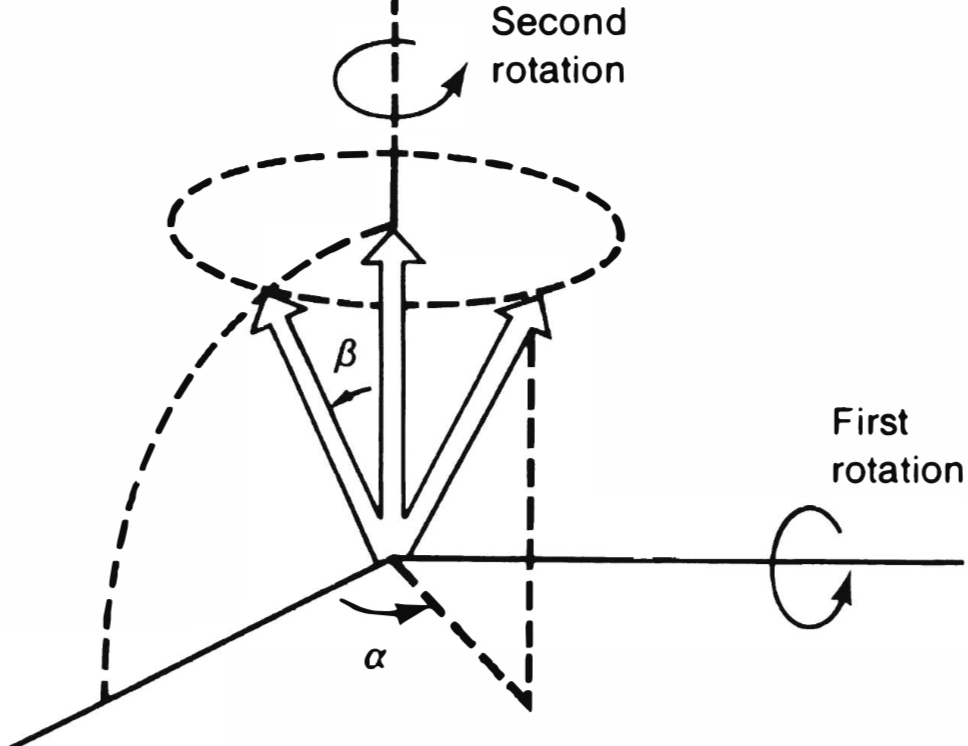
\includegraphics[width=7cm]{AngularMomentum/alphabeta.png}
\caption{倾角$\alpha$和方位角$\beta$的定义。}
%\label{default}
\end{center}
\end{figure}

假设$\hat n$的取向用如图$\alpha$,$\beta$两个角来表示,即$\hat n$的取向由$\hat z$出发,先倒下一个倾角$\alpha$,再在$x-y$平面上转过一个方位角$\alpha$。

$S_n$是延$\hat n$方向的,其本征值问题是:

\begin{equation}
S_n \left| n,+ \right\rangle = \frac{\hbar }{2} \left| n,+ \right\rangle
\end{equation}

这里的$\left| n,+ \right\rangle$可看做是对$S_z$的本征矢$\left| + \right\rangle$先围绕$y$轴转$\beta$角度,再围绕$z$轴转$\alpha$角度。

\begin{equation}
\left| n,+ \right\rangle = e^{- \frac{ i S_z \alpha }{ \hbar }}  e^{- \frac{ i S_y \beta }{ \hbar }}  \left| + \right\rangle
\end{equation}

这里我们规定:$U = e^{- \frac{ i S_z \alpha }{ \hbar }}  e^{- \frac{ i S_y \beta }{ \hbar }}$。

$S_z$的本征值问题可改写为:

\begin{equation}
U S_z U^\dagger U \left| + \right\rangle = \frac{\hbar}{2} U \left| + \right\rangle
\end{equation}

即:

\begin{equation}
S_n = U S_z U^\dagger
\end{equation}

或改写为泡利矩阵的形式:

\begin{equation}
\sigma_n = U \sigma_z U^\dagger
\end{equation}

即:

\begin{equation}
\sigma_n = e^{- \frac{ i \sigma_z \alpha }{2}} e^{- \frac{ i \sigma_y \beta }{2}} \sigma_z e^{ \frac{ i \sigma_y \beta }{2}}  e^{ \frac{ i \sigma_z \alpha }{2}}
\end{equation}

展开后可得:

\begin{equation}
\sigma_n = \left( \begin{array}{cc}  \cos \beta & \sin \beta e^{- i \alpha}  \\  \sin \beta e^{i \alpha} & - \cos \beta  \end{array}  \right)
\end{equation}

在$\hat n$方向旋转$\phi$角度的变换矩阵为:

\begin{equation}
e^{- \frac{ i \sigma_n \phi}{2}} = 1 \cos \left( \frac{\phi}{2} \right) - i \sigma_n \sin \left( \frac{\phi}{2}  \right) 
\end{equation}

上式中的$1$表示单位算符,计算可得:

\begin{equation}
e^{- \frac{ i \sigma_n \phi}{2}} = \left( \begin{array}{cc}   \cos \frac{\phi}{2} - i \cos \beta \sin \frac{\phi}{2} & - i \sin \beta e^{- i \alpha} \sin \frac{\phi}{2} \\  - i \sin \beta e^{i \alpha} \sin \frac{\phi}{2} & \cos \frac{\phi}{2} + i \cos \beta \sin \frac{\phi}{2}   \end{array}  \right)
\end{equation}

考虑到单位向量$\hat n$在$x$, $y$和$z$轴的投影:

\begin{eqnarray}
n_x & = & \sin \beta \cos \alpha \\
n_y & = & \sin \beta \sin \alpha \\
n_z & = & \cos \beta
\end{eqnarray}

$e^{- \frac{ i \sigma_n \phi}{2}}$可表示为:

\begin{equation}
e^{- \frac{ i \sigma_n \phi}{2}} = \left( \begin{array}{cc}   \cos \frac{\phi}{2} - i n_z \sin \frac{\phi}{2} & \left( - i n_x - n_y  \right) \sin \frac{\phi}{2} \\  \left( - i n_x + n_y  \right) \sin \frac{\phi}{2} & \cos \frac{\phi}{2} + i n_z \sin \frac{\phi}{2}   \end{array}  \right)
\end{equation}

所有这样的操作构成了一个幺正幺模群\index{Unitary unimodular group:幺正幺模群}(Unitary unimodular group),幺正条件是$U^\dagger U = 1$,幺模条件是$\det U = 1$(泡利矩阵$\sigma_x$等就不满足幺模条件)。

一个二维幺正幺模的矩阵可表示为:

\begin{equation}
U(a,b)=\left( \begin{array}{cc}  a & b \\ - b^* & a^*  \end{array} \right)
\end{equation}

同时必须满足:

\begin{equation}
|a|^2 + |b|^2 = 1
\end{equation}

我们把二维的幺正幺模群记为SU(2),这里的S表示Special。值得注意的是,尽管SU(2)和SO(3)都可用以表示三维实空间中的转动,但它们并不是同构的(isomorphic)。考虑一个$\phi = 2 \pi$的旋转和一个$4 \pi$的旋转,对SO(3)我们得到相同的矩阵元,但对SU(2)则正好差一个负号,但我们可以构造U(a,b)或U(-a,-b)到SO(3)的一一对应,在此意义上我们说它们是局域同构的(locally isomorphic)。

\subsection{欧拉转动}

三维实空间(物理空间)中的转动可以用三个参量来表示(比如$\hat n (\beta, \alpha)$和$\phi$),我们也可以用欧拉转动\index{Euler Rotations:欧拉转动}(Euler Rotations)来表示。

欧拉转动($\alpha, \beta, \gamma$)的定义如图:

\begin{figure}[htbp]
\begin{center}
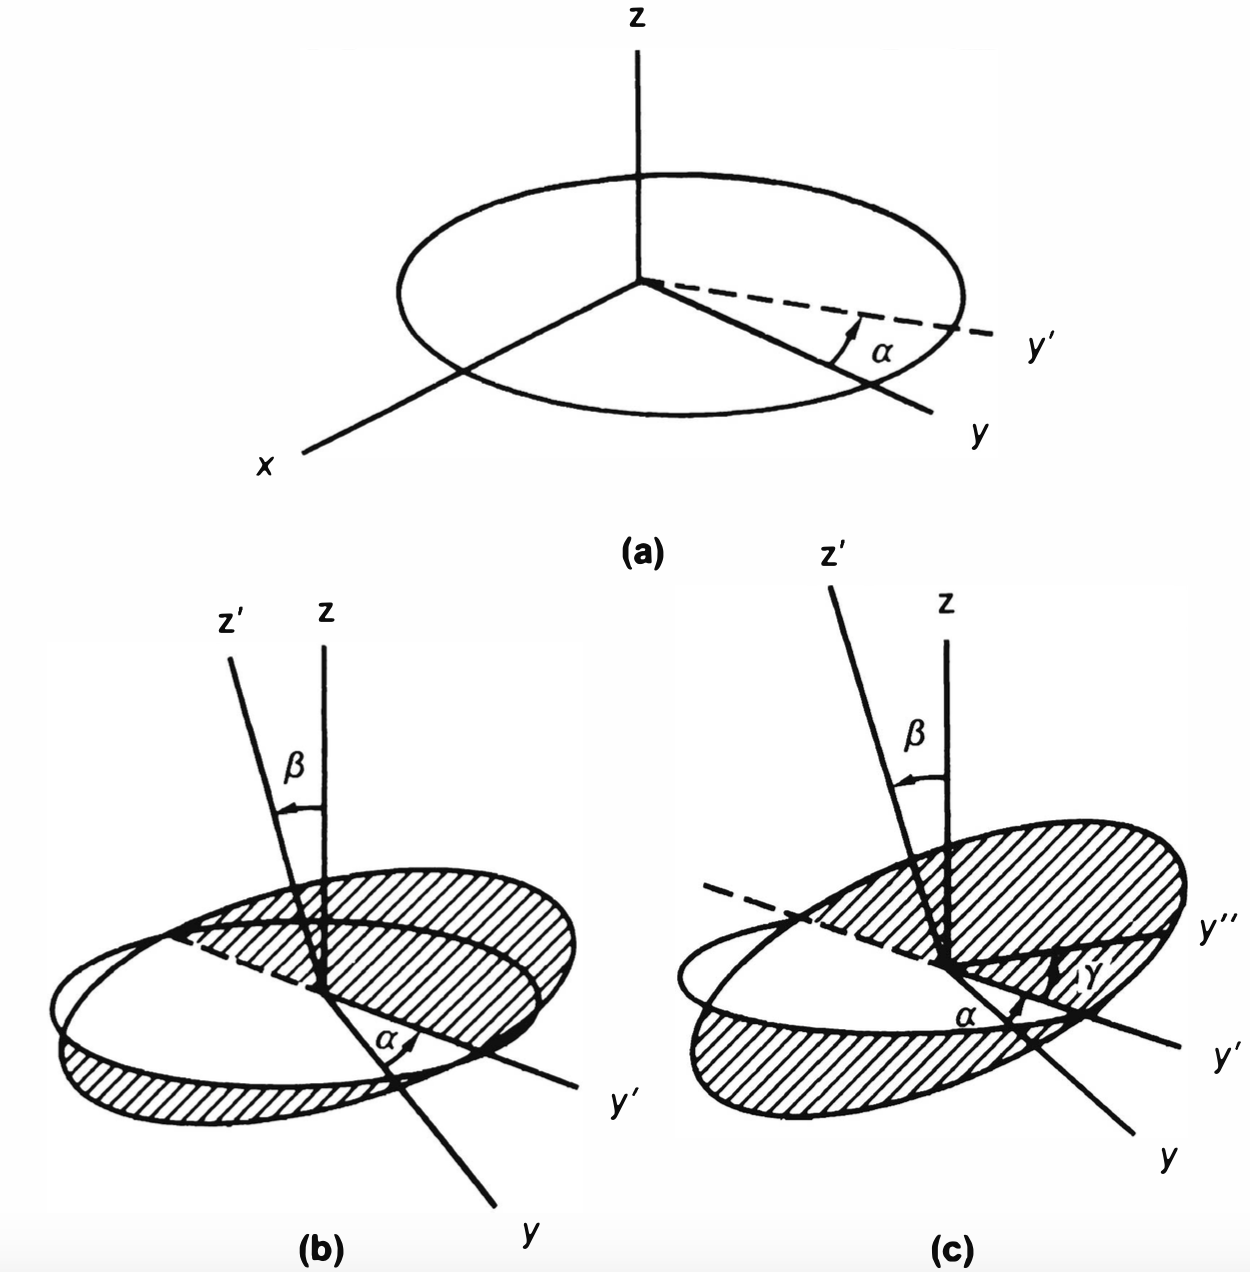
\includegraphics[width=10cm]{AngularMomentum/eulerrotations.png}
\caption{欧拉转动}
%\label{default}
\end{center}
\end{figure}

首先我们要注意区分两种坐标系,一种是空间固定的(space-fixed)坐标系,用$O-xyz$表示,另一种是物体固定的(body-fixed)坐标系,用$O-x' y' z'$等表示。

欧拉转动$R(\alpha, \beta, \gamma)$被定义为(a)围绕空间固定的$z$轴转$\alpha$角;然后(b)围绕物体固定的$y'$轴转$\beta$角,注意此时$y'$轴和空间固定的$y$轴已经不重合了,相差有$\alpha$角;最后(c)围绕物体固定的$z'$轴转$\gamma$角,这个$z'$轴和$z$轴相差$\beta$角。

\begin{equation}
R(\alpha, \beta, \gamma) = R_{z'}(\gamma) R_{y'} (\beta) R_z (\alpha)
\end{equation}

可以验证各个转动间存在着这样的关系:

\begin{equation}
R_{y'}(\beta) = R_z (\alpha) R_y (\beta) R_z^{-1}(\alpha)
\end{equation}

这里$R^{-1}$表示“反方向”转,通过使一个扁平物体按步骤转起来不难证明以上关系。类似地,我们还有:

\begin{equation}
R_{z'}(\gamma) = R_{y'} (\beta) R_z (\gamma) R_{y'}^{-1}(\beta)
\end{equation}

由以上两个关系,我们可以证明:

\begin{eqnarray*}
R_{z'} (\gamma) R_{y'} (\beta) R_z (\alpha) & = &  R_{y'} (\beta) R_z (\gamma) R_{y'}^{-1}(\beta) R_{y'} (\beta) R_z (\alpha) \\
{} & = & R_{y'} (\beta) R_z (\gamma) R_z (\alpha) \\
{} & = & R_z (\alpha) R_y (\beta) R_z^{-1}(\alpha) R_z (\gamma) R_z (\alpha) \\
{} & = & R_z (\alpha) R_y (\beta) R_z (\gamma)
\end{eqnarray*}

由以上关系,我们可得到在态空间中转动的算符的关系:

\begin{equation}
D(\alpha, \beta, \gamma ) = D_z (\alpha) D_y (\beta) D_z (\gamma)
\end{equation}

现在所有转动($\alpha$,$\beta$和$\gamma$)都是针对空间固定的转轴进行的。

\subsection*{参考}

J. J. Sakurai, Modern Quantum Mechanics, \S 3.1, 3.2, 3.3



\section{角动量相加}

\subsection{直积空间}

我们曾在原子物理中接触过两个角动量相加的例子,一个是电子的“自旋-轨道”耦合即电子的轨道角动量和电子的自旋角动量相加;一个是两个电子的自旋角动量相加。两个电子的自旋是独立的自由度,即第一个电子自旋的状态与第二个电子自旋的状态无关;对“自旋-轨道”耦合而言,电子的轨道运动和电子自旋的状态也是无关的。

这意味着我们可以用直积\index{direct product:直积}(direct product)空间去表示两个电子的自旋或电子的“自旋-轨道”耦合的态。直积空间的想法很简单,就是把两个独立自由度的元素并列,我们约定好前面的元素表示第一个自由度,后面的元素表示第二个自由度。

\begin{equation}
A \otimes B = \{ a_i \} \otimes \{ b_j \} =  \{ a_i b_j \}
\end{equation}

对直积空间$A \otimes B$而言,$A \otimes B$的维度等于集合$A$的维度乘以集合$B$的维度。比如对两个自旋1/2组成的系统,复系数线性向量空间就是4维的,4个基矢分别为:

\begin{equation*}
\left| ++ \right\rangle, \left| +- \right\rangle, \left| -+ \right\rangle, \left| -- \right\rangle 
\end{equation*}

第一个基矢的意思就是第一个自旋向上,而第二个自旋向下。两个自旋组成系统的任意态矢可以表示为以上四个基矢的线性叠加。

对“自旋-轨道”耦合问题来说,因轨道部分基矢不是可数的,因此显得更抽象。

\begin{equation}
\{ \left| x' \right\rangle  \} \otimes \{  \left| + \right\rangle , \left| - \right\rangle   \}
\end{equation}

这里空间部分取位置算符本征矢$\left| x' \right\rangle $为基矢。其“个数”为不可数的无穷多(或用数学的名称说是“阿列夫1”个)。

在想象中,所有这样的基矢(共“2倍阿列夫1”个)可表示为如下两个系列:

\begin{eqnarray*}
\left| x', +  \right\rangle, \left| x'', +  \right\rangle, \left| x''', +  \right\rangle ... \\
\left| x', -  \right\rangle, \left| x'', -  \right\rangle, \left| x''', -  \right\rangle ...
\end{eqnarray*}

任意态矢$\left| \alpha \right\rangle$可表示为以上所有基矢的线性叠加,叠加因子可表示为:

\begin{eqnarray*}
\left\langle x', + | \alpha \right\rangle, \left\langle x'', + | \alpha \right\rangle, \left\langle x''', + | \alpha \right\rangle ... \\
\left\langle x', - | \alpha \right\rangle, \left\langle x'', - | \alpha \right\rangle, \left\langle x''', - | \alpha \right\rangle ...
\end{eqnarray*}

把这一系列迭加因子连续化,上一行对应的就是$ \psi_+(x) =  \left\langle x, + | \alpha \right\rangle $,下一行是$\psi_-(x) = \left\langle x, - | \alpha \right\rangle$,即自旋向上和向下的波函数,写成列向量的形式:

\begin{equation}
\left( \begin{array} {c}  \psi_+(x)  \\  \psi_-(x)  \end{array}  \right)
\end{equation}

\subsection{角动量相加的定义}

我们一般把两角动量相加写成如下的矢量相加的形式:

\begin{equation}
J = L + S
\end{equation}

但想想这么写有点别扭,因为轨道角动量$L$作用在轨道自由度,自旋角动量作用于自旋自由度,这两个自由度是独立的,并非同类,如何相加?

更加严谨的定义是:

\begin{equation}
J = L \otimes 1 + 1 \otimes S
\end{equation}

即总角动量$J$是定义在轨道自由度和自旋自由度的直积空间上的,这样左右就都是定义在相同空间上的算符了。

对应的转动算符是:

\begin{equation}
D(R) = D^{orb}(R) \otimes D^{spin} (R)
\end{equation}

无穷小转动:

\begin{equation}
\left( 1- \frac{i J_1 \cdot \hat n \delta \phi}{ \hbar}   \right) \otimes \left( 1- \frac{i J_2 \cdot \hat n \delta \phi}{ \hbar}   \right) = 1 - \frac{ i \left( J_1 \otimes 1 + 1 \otimes J_2  \right) \cdot \hat n \delta \phi }{ \hbar}
\end{equation}

\subsection{CG系数}

求解量子力学的核心是找到一组两两都对易的最大的力学量完全集,这意味着我们可以用其共同的本征矢来构造有物理含义的基矢。对两个角动量$J_1$和$J_2$相加的问题,我们发现我们有两套力学量完全集可供选择,即我们有两套基矢,它们分别对不同的问题最好用。我们现在的任务是求出这两套基矢(表象)之间的变换矩阵,而这些矩阵元就叫CG系数。

一套基矢的选择是基于完全集$( J_1^2, J_2^2, J_{1z}, J_{2z}  )$:

\begin{eqnarray}
J_1^2 \left|j_1 j_2 ; m_1 m_2 \right\rangle & = &  j_1 (j_1 +1 )\hbar^2  \left|j_1 j_2 ; m_1 m_2 \right\rangle \\
J_2^2 \left|j_1 j_2 ; m_1 m_2 \right\rangle & = &  j_2 (j_2 +1 )\hbar^2  \left|j_1 j_2 ; m_1 m_2 \right\rangle \\
J_{1z} \left|j_1 j_2 ; m_1 m_2 \right\rangle & = & m_1 \hbar \left|j_1 j_2 ; m_1 m_2 \right\rangle \\
J_{2z} \left|j_1 j_2 ; m_1 m_2 \right\rangle & = & m_2 \hbar \left|j_1 j_2 ; m_1 m_2 \right\rangle
\end{eqnarray}

其特点是我们可以说清$J_1$和$J_2$所处的状态,即$j_{1z} = m_1$和$j_{2z} = m_2$,我们称这套表象为$m_1 m_2$表象。

第二套基矢的选择是基于完全集$( J^2, J_1^2, J_2^2, J_z )$:

\begin{eqnarray}
J_1^2 \left|j_1 j_2 ; jm \right\rangle & = &  j_1 (j_1 +1 )\hbar^2  \left|j_1 j_2 ; jm \right\rangle \\
J_2^2 \left|j_1 j_2 ; jm \right\rangle & = &  j_2 (j_2 +1 )\hbar^2  \left|j_1 j_2 ; jm \right\rangle \\
J^2 \left|j_1 j_2 ; jm \right\rangle & = & j (j + 1) \hbar^2 \left|j_1 j_2 ; jm \right\rangle \\ 
J_{z} \left|j_1 j_2 ; jm \right\rangle & = & m \hbar \left|j_1 j_2 ; jm \right\rangle
\end{eqnarray}

这里$J_z = j$是总角动量的第3分量,即我们可以说清总角动量$J$所处的状态,我们称这套表象为$jm$表象。

上述两套基矢的变换关系可表示为:

\begin{equation}
\left| jm \right\rangle = \sum\limits_{m_1, m_2} \left|  m_1 m_2  \right\rangle \left\langle m_1 m_2 | j m \right\rangle
\end{equation}

这里$\left\langle m_1 m_2 | j m \right\rangle$就是CG系数\index{CG coefficients:CG系数}。

由角动量相加的“矢量模型”\index{vector model of angular momentum:角动量的矢量模型},我们可以很直观地“猜测出”CG系数应有的两个性质:

(1)除了符合$m = m_1 + m_2$条件外的CG系数都为0。

证明如下,首先:

\begin{equation}
J_z = J_{1z} + J_{2z}
\end{equation}

这意味着:

\begin{equation}
(J_z - J_{1z} - J_{2z}) \left| jm \right\rangle = 0
\end{equation}

左乘$\left\langle m_1 m_2 \right|$,得到:

\begin{equation}
( m - m_1 - m_2) \left\langle m_1 m_2 | j m \right\rangle = 0 
\end{equation}

这意味着我们只需要考虑$m = m_1 + m_2$这样的CG系数。

(2)除非满足$| j_1 - j_2 | \le j \le j_1 + j_2$否则CG系数为0。

从“矢量模型”的角度看,该性质是非常直观的。(三角形的一条边大于两邻边的差,同时小于两邻边的和。)

严格地证明此性质比较啰嗦,但我们可以如下说明此性质是合理的。

两角动量相加,总量子数$j$的取值范围是:

\begin{equation*}
|j_1 - j_2|, |j_1 - j_2|+1 , ... , j_1 + j_2 -1, j_1 + j_2
\end{equation*}

对每一个固定的$j$,有$2j+1$个本征态($-j, -j+1, ..., j-1, j$)。把所有独立的本征态都加起来,就是$(2j_1 + 1) (2 j_2 +1)$个。这意味着角动量量子数分别为$j_1$和$j_2$的两角动量相加构成了一个$(2j_1 + 1) (2 j_2 +1)$维的希尔伯特空间,这和把$J_1$、$J_2$分别看作是两个独立的自由度,构成直积空间所得的维度是一样的。

(3)CG系数构成一个幺正矩阵$U U^\dagger = 1$。如果我们进一步约定CG系数取实数的话(这意味着 $U U^T =1$,即变换矩阵是个正交矩阵 ),我们会得到一个归一关系。

首先:

\begin{equation}
\sum\limits_{jm}  \left\langle m_1 m_2 | j m \right\rangle \left\langle jm | m_1' m_2' \right\rangle = \delta_{m_1 m_1' } \delta_{ m_2 m_2'} 
\end{equation}

约定CG系数为实:$ \left\langle jm | m_1' m_2' \right\rangle  = \left\langle  m_1' m_2' | jm \right\rangle $,于是:

\begin{equation}
\sum\limits_{jm}  \left\langle m_1 m_2 | j m \right\rangle \left\langle m_1' m_2' | j m \right\rangle = \delta_{m_1 m_1' } \delta_{ m_2 m_2'} 
\end{equation}

类似地,

\begin{equation}
\sum\limits_{m_1 m_2}  \left\langle jm | m_1 m_2 \right\rangle \left\langle m_1 m_2 | j' m' \right\rangle = \delta_{jj' } \delta_{ mm'} 
\end{equation}

令$j' = j$,$m' = m = m_1 + m_2  $,得到:

\begin{equation}
\sum\limits_{m_1 m_2} \left\langle m_1 m_2 | j m \right\rangle^2 = 1
\end{equation}

假如我们把所有CG系数都用某个CG系数表示,我们就能通过上式具体定下来各个CG系数的取值。

\subsection{CG系数的求解}

回忆我们是如何研究两个自旋1/2的物理系统的。首先我们猜测$\left| ++ \right\rangle$对应$j=1$,$m=1$的态,然后我们用降算符$S^- = S_1^- + S_2^-$作用于它,然后利用关系:

\begin{equation}
J_{\pm} \left| j,m \right\rangle = \hbar \sqrt{ (j \mp m ) ( j \pm m + 1 ) } \left| j,m \pm 1 \right\rangle
\end{equation}

对$\left| j=1, m=1  \right\rangle = \left|  +  +  \right\rangle$ 进行运算,即可得到$\left| j = 1, m=0  \right\rangle $与$\left|  -  +  \right\rangle$和$\left|  +  -  \right\rangle$的表达式,……

现在我们从$jm$表象下的某个态$\left| jm \right\rangle$出发,类似地操作:

\begin{equation}
J_{\pm} \left| jm \right\rangle = (J_{1 \pm} + J_{2 \pm}) \sum\limits_{m_1 m_2} \left| m_1 m_2  \right\rangle \left\langle m_1 m_2 | jm \right\rangle
\end{equation}

利用$J_{\pm}$的关系可得:

\begin{eqnarray*}
\sqrt{...} \left| j, m \pm 1 \right\rangle & = & \sum\limits_{m_1' m_2'}  \left( \sqrt{...} \left| m_1' \pm 1 , m_2' \right\rangle + \sqrt{...} \left| m_1', m_2' \pm 1 \right\rangle \right) \\
{} & {} &  \times \left\langle m_1' m_2' | j m \right\rangle
\end{eqnarray*}

这里$\sqrt{...}$是系数,$m_1 \to m_1' $,$m_2 \to m_2'$,$\sum\limits_{m_1 m_2 } \to \sum\limits_{m_1' m_2' }$。

等式两边左乘$\left\langle m_1 m_2 \right|$,

\begin{eqnarray*}
{} & {} & ...\left\langle m_1 m_2 | j, m \pm 1 \right\rangle \\
{} & = &  \sum\limits_{m_1' m_2'} \left( ... \left\langle m_1 m_2 | m_1' \pm 1 , m_2' \right\rangle  + ... \left\langle m_1 m_2 | m_1', m_2' \pm 1 \right\rangle  \right) \\
{} & {} & \times \left\langle m_1' m_2' | j m \right\rangle 
\end{eqnarray*}

$\left\langle m_1 m_2 | m_1' \pm 1 , m_2' \right\rangle = \delta_{m_1, m_1' \pm 1 }  \delta_{m_2 , m_2'} $意味着:

\begin{eqnarray*}
m_1 & = & m_1' \pm 1 \\
m_2 & = & m_2'
\end{eqnarray*}

即:

\begin{eqnarray*}
m_1' & = & m_1 \mp 1 \\
m_2' & = & m_2
\end{eqnarray*}

$\left\langle m_1 m_2 | m_1', m_2' \pm 1 \right\rangle = \delta_{m_1 , m_1'} \delta_{m_2 , m_2'  \pm 1}$意味着:

\begin{eqnarray*}
m_1 & = & m_1' \\
m_2 & = & m_2'  \pm 1
\end{eqnarray*}

即:

\begin{eqnarray*}
m_1' & = & m_1 \\
m_2' & = & m_2  \mp 1
\end{eqnarray*}

最终我们将得到:

\begin{equation}
... \left\langle m_1 m_2 | j, m \pm 1 \right\rangle = ... \left\langle m_1 \mp 1, m_2 | j m \right\rangle + ... \left\langle m_1,  m_2 \mp 1  | j m \right\rangle
\end{equation}

上符号(upper sign)对应$J_+$关系,下符号(lower sign)对应$J_-$关系。我们可把这两个关系放到$m_1  m_2$平面上去。

\begin{figure}[htbp]
\begin{center}
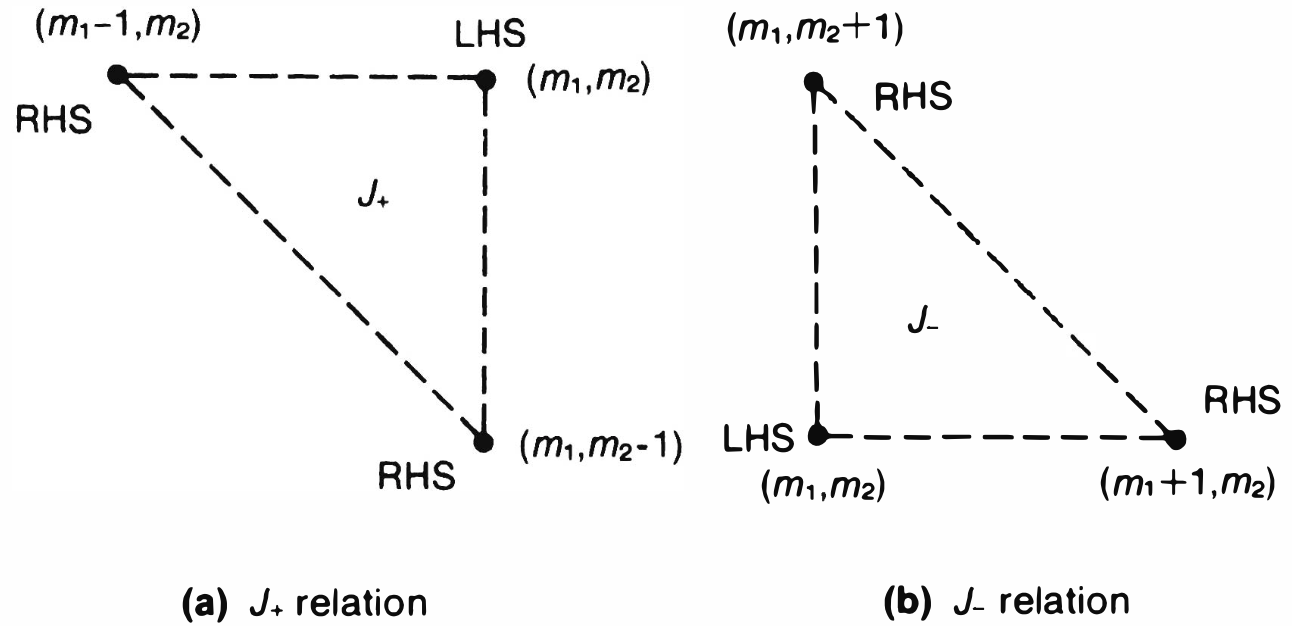
\includegraphics[width=10cm]{AngularMomentum/J+J-relation}
\caption{左图是$J_+$关系,右图是$J_-$关系。分别联系起三个不同的CG因子。}
%\label{default}
\end{center}
\end{figure}

这里$m_1 = -j_1, -j_1 + 1, ..., j_1 -1, j_1$,即在$-j_1$到$j_1$之间间隔为1的分立取值,类似地$m_2$是$-j_2$到$j_2$之间间隔为1的分立取值。如果我们取$m_1$为横轴,$m_2$为纵轴,$(m_1, m_2)$就构成了$m_1  m_2$平面上的一系列格点。每一个格点都代表一个CG系数$\left\langle m_1 ,  m_2 | j, m_1 + m_2 \right\rangle$。

现在我们就可给出角动量$j_1$加角动量$j_2$的所有CG系数的一般步骤。

(1)$j = |j_1 - j_2|, ... j_1 + j_2 -1, j_1 + j_2$;

(2)对某个确定的$j$,$m_1 + m_2  = - j, -j +1, ..., j$;所有非零CG系数被包围在$m_1 = \pm j_1$,$m_2 = \pm j_2$和$m_1 + m_2 = \pm j$这六条直线围成的多边形内。

\begin{figure}[htbp]
\begin{center}
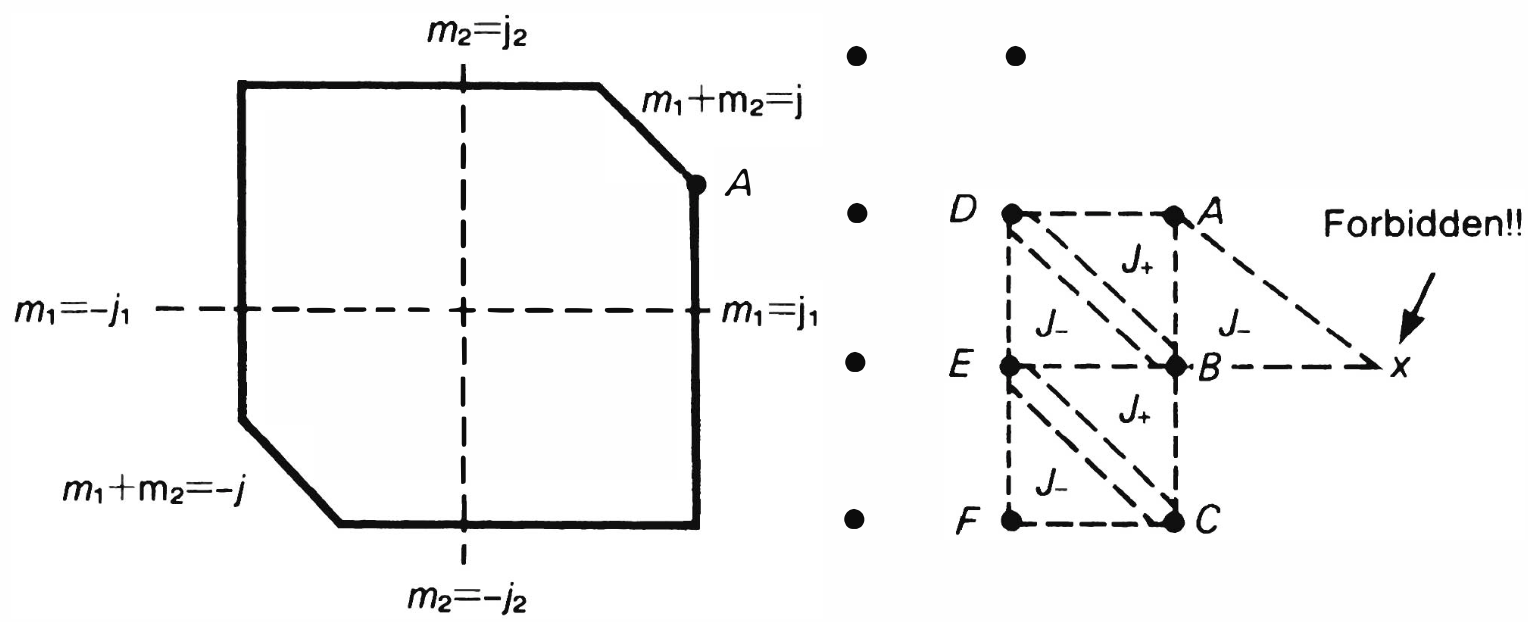
\includegraphics[width=10cm]{AngularMomentum/cgcoeficients.png}
\caption{左图:CG系数不为零的区域;右图:利用$J_{\pm}$关系“递推”CG系数。}
\label{default}
\end{center}
\end{figure}

(3)我们由图中的A点出发,首先构造$J_-$三角形ABX,由于X已经出了CG系数不为零的区域,所以该点的CG系数为0,这样我们就能用A点的CG系数表示B点的CG系数了。然后我们再构造$J_+$三角形ABD,这样D点的CG系数也可以用A点的CG系数来表示了。我们可以一直这么做下去,……直到覆盖整个CG系数不为0的区域,最后再利用归一关系把各点CG系数的取值最终确定下来。


\subsection*{参考}

J. J. Sakurai, Modern Quantum Mechanics, \S 3.5, 3.6, 3.7, 3.8


\section{对称性}

\subsection{守恒量}

迄今为止我们已经研究过空间平移对称、时间平移对称和旋转对称。这些对称操作可用一个(或一组)连续参量来表示,参量取值与对称操作有一一对应的关系,参量的连续变化描述了群元的连续变化,如此构成的群是个连续群。群元乘积的参量是每个操作参量的单值解析函数,这样的连续群称为李群(Lie Group)。这里我们只是提及这些名词,并不深入数学上的细节。

我们用一个幺正算符$U$来表示对称操作中的一个元素,对无穷小参量$\epsilon$,可统一写成如下形式:

\begin{equation}
U(\epsilon) = 1 - \frac{i \epsilon G}{\hbar}
\end{equation}

$G^\dagger = G$是厄米算符,是对称算符的产生算符,因为我们只要让很多无穷小算符连乘就可得到有限参量的对称操作。$G$可以是$p_x$,$H$或$J_z$,对应的无穷小参量是$\delta x$,$\delta t$和$\delta \phi$。

在对称操作$U$下,态矢量$\left| \alpha \right\rangle \to U \left| \alpha \right\rangle $,假设在对称操作$U$下,哈密顿$H$是不变的。这意味着:

\begin{equation}
\left\langle \alpha \right| H \left| \alpha \right\rangle = \left\langle \alpha \right| U^\dagger H U \left| \alpha \right\rangle 
\end{equation}

即:$H = U^\dagger H U$,那么:$U H = H U $,那么:

\begin{equation*}
\left( 1 - \frac{i \epsilon G}{\hbar} \right) H = H \left( 1 - \frac{i \epsilon G}{\hbar} \right)
\end{equation*}

这意味着:

\begin{equation}
[G, H ] = 0
\end{equation}

考虑海森堡运动方程\index{Heisenberg equation of motion:海森堡运动方程}:

\begin{equation}
i \hbar \dot G = [G, H ] = 0
\end{equation}

这意味着力学量$G$是守恒量。即空间平移对称对应“动量守恒”,时间平移对称对应“能量守恒”,而转动对称对应“角动量守恒”。

假设$\left| n \right\rangle$是$H$的本征态,对应的本征值是$E_n$

\begin{equation}
H \left| n \right\rangle = E_n \left| n \right\rangle
\end{equation}

由于$ HU = UH$,

\begin{equation}
H U \left| n \right\rangle = U H \left| n \right\rangle = E_n U \left| n \right\rangle 
\end{equation}

即$U \left| n \right\rangle $和$\left| n \right\rangle$都对应相同的能量本征值$E_n$,如果$U \left| n \right\rangle $和$\left| n \right\rangle$是两个不同的量子态,我们就说$E_n$是简并的。

\subsection{宇称}

除了连续的对称操作,还有分立的对称操作。比如宇称\index{Parity:宇称}(parity,也叫空间反演),

\begin{equation}
\left| \alpha \right\rangle \to \pi \left| \alpha \right\rangle
\end{equation}

使得:

\begin{equation}
\left\langle x \right\rangle \to  \left\langle \alpha \right| \pi^\dagger x \pi \left| \alpha \right\rangle   =  - \left\langle  \alpha \right|  x \left| \alpha \right\rangle 
\end{equation}

这意味着:

\begin{equation}
\pi^\dagger x \pi = - x 
\end{equation}

我们说位置矢量$x$在宇称变换下是奇(odd)的。

现在考虑如图操作:

\begin{figure}[htbp]
\begin{center}
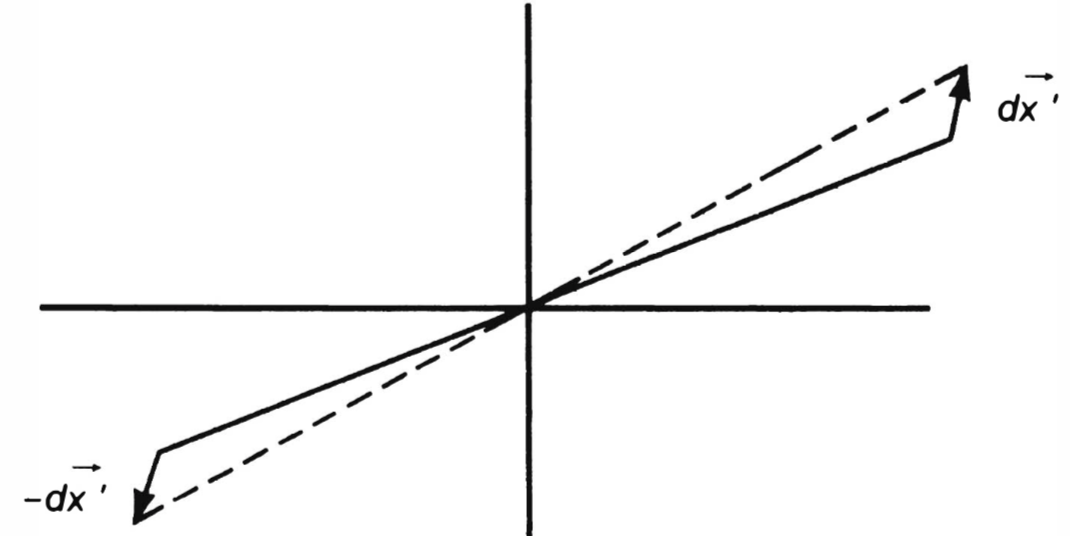
\includegraphics[width=9cm]{Symmetry/piTTpi.png}
\caption{$\pi T(dx') = T(- dx') \pi$}
%\label{default}
\end{center}
\end{figure}

先平移$T(dx')$再宇称(空间反演\index{inversion:空间反演},inversion)$\pi$的效果$\pi T(dx')$和先宇称$\pi$再反方向平移$T(- dx')$的效果$ T(- dx') \pi$是一样的。记作:

\begin{equation}
\pi T(dx') = T(- dx') \pi
\end{equation}

这意味着:

\begin{equation}
\pi \left( 1 - \frac{i p dx'}{\hbar}   \right) = \left( 1 + \frac{i p dx'}{\hbar}   \right) \pi
\end{equation}

即:

\begin{equation}
\pi^\dagger p \pi = - p
\end{equation}

动量算符在宇称变换下也是奇(odd)的。

现在来考虑角动量算符$J$,对轨道角动量$L = x \times p$,我们猜测角动量在宇称变换下是偶(even)的。

在三维实空间,空间反演(即宇称变换)可写为:

\begin{equation}
R(\pi) = \left( \begin{array}{ccc} -1 & 0 & 0 \\ 0 & -1 & 0 \\ 0 & 0 & -1  \end{array}  \right)
\end{equation}

$R(\pi)$与实空间中的任意转动$R_{n} (\phi)$对易:

\begin{equation}
R(\pi) R_{n} (\phi) = R_{n} (\phi) R(\pi)
\end{equation}

对应到态矢空间中的变换矩阵应有相同的关系:

\begin{equation}
\pi D(R) = D(R) \pi
\end{equation}

这意味着:

\begin{equation}
\pi \left( 1- \frac{i J_n d \phi}{\hbar}  \right) = \left( 1- \frac{i J_n d \phi}{\hbar}  \right) \pi
\end{equation}

即:

\begin{equation}
\pi^\dagger J_n \pi = J_n 
\end{equation}

我们称$x$,$p$这样的向量叫极向量\index{polar vector:极向量}(polar vector),而称像角动量$J$这样的向量为轴向量\index{axial vector:轴向量}(axial vector),或赝向量\index{pseudovector:赝向量}(pseudovector)。在此基础上我们可继续定义标量,如$L \cdot S$和赝标量\index{pseudoscalar:赝标量}$S \cdot x$。

\begin{eqnarray}
\pi^\dagger L \cdot S  \pi & = & L \cdot S \\
\pi^\dagger  S \cdot x  \pi & = & - S \cdot x
\end{eqnarray}

练习:假设$[H, \pi] = 0$(哈密顿具有宇称对称),假设$\left| n \right\rangle$是$H$的非简并本征态(nondegenerate eigenket),对应本征值是$E_n$,求证$\left| n \right\rangle$也是宇称算符$\pi$的本征态。

Prove:首先构造态矢量

\begin{equation}
\frac{ \left| n \right\rangle \pm \pi \left| n \right\rangle }{2}
\end{equation}

它是宇称算符的本征态,

\begin{equation}
\pi \left( \frac{ \left| n \right\rangle \pm \pi \left| n \right\rangle }{2}  \right) = \frac{ \pi \left| n \right\rangle \pm \left| n \right\rangle }{2} = \pm \frac{\left| n \right\rangle \pm \pi \left| n \right\rangle}{2}
\end{equation}

其本征值是$\pm 1$,并且这个态对应能量本征值仍然是$E_n$:

\begin{equation}
H \frac{ \left| n \right\rangle \pm \pi \left| n \right\rangle }{2} = E_n \frac{ \left| n \right\rangle \pm \pi \left| n \right\rangle }{2}
\end{equation}

由于$E_n$非简并,$\frac{ \left| n \right\rangle \pm \pi \left| n \right\rangle }{2}$实际上和$\left| n \right\rangle$是一个态(可以相差一个相位因子)。

\subsection{对称双井}

考虑如图“左右对称”的双井,它符合上述$[ H, \pi ] = 0$的条件,其能量本征态$\left| n \right\rangle$具有确定的奇偶性。考虑能量最低“偶宇称”的态$\left| S \right\rangle$,其能量本征值是$E_S$,和能量最低“奇宇称”的态$\left| A \right\rangle$,其能量本征值是$E_A$。

\begin{figure}[htbp]
\begin{center}
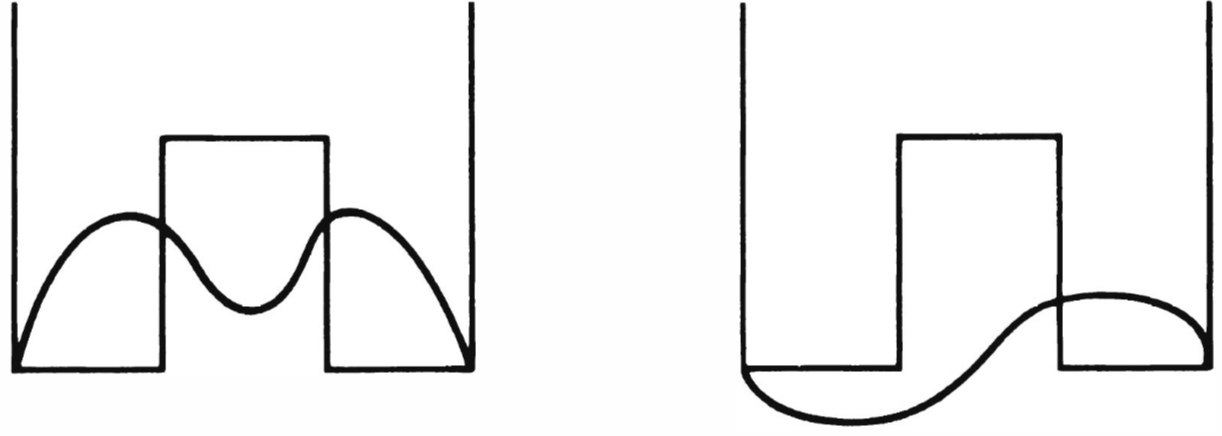
\includegraphics[width=8cm]{Symmetry/symmetry-antisymmetry.png}
\caption{左:偶宇称的态;右:奇宇称的态。}
%\label{default}
\end{center}
\end{figure}

由于奇宇称的态$\left| A \right\rangle$起伏更激烈,所以有

\begin{equation}
E_A > E_S
\end{equation}

假设对称双井中间的势垒较高,即$\left| S \right\rangle$和$\left| A \right\rangle$在左井和右井中“波函数的形状”大致相同。这样我们可以把$\left| S \right\rangle$和$\left| A \right\rangle$组合起来分别得到局域在右井和左井中的态矢量$\left| R \right\rangle$和$\left| L \right\rangle$:

\begin{eqnarray}
\left| R \right\rangle  & = & \frac{ \left| S \right\rangle + \left| A \right\rangle  }{\sqrt{2}} \\
\left| L \right\rangle & = & \frac{ \left| S \right\rangle - \left| A \right\rangle  }{\sqrt{2}}
\end{eqnarray}

假设$t=0$,粒子处于右井中,即$\left| R, t=0 \right\rangle$,态矢量将如何演化?考虑:

\begin{eqnarray*}
\left| R , t \right\rangle & = & e^{- \frac{iHt}{\hbar}}  \left| R \right\rangle =  \frac{ e^{- \frac{iHt}{\hbar}} \left| S \right\rangle + e^{- \frac{iHt}{\hbar}} \left| A \right\rangle   }{\sqrt 2} \\
{} & = & \frac{ e^{- \frac{iE_S t}{\hbar}} \left| S \right\rangle + e^{- \frac{i E_A t}{\hbar}} \left| A \right\rangle   }{\sqrt 2} \\
{} & = & \frac{1}{\sqrt 2} e^{ - \frac{i E_S t}{ \hbar} } \left( \left| S \right\rangle + e^{- \frac{i (E_A - E_S) t }{ \hbar}}  \left| A \right\rangle  \right)
\end{eqnarray*}

由上式括号中第二项可看出,每经历半周期$\left| R \right\rangle \to \left| L \right\rangle $,再经历半周期$\left| L \right\rangle \to \left| R \right\rangle $,即粒子会经历从右井到左井,再从左井回到右井的反复周期振荡。振荡周期为:

\begin{equation}
T = \frac{h }{E_A - E_S}
\end{equation}

由上式可见,$E_A$和$E_S$越接近,粒子由右井振荡到左井的时间就越久,如果$E_A$无限趋近于$E_S$,粒子就会“永远”呆在右井。对应就是对称双井中间的势垒趋于无限高的情形。

\begin{figure}[htbp]
\begin{center}
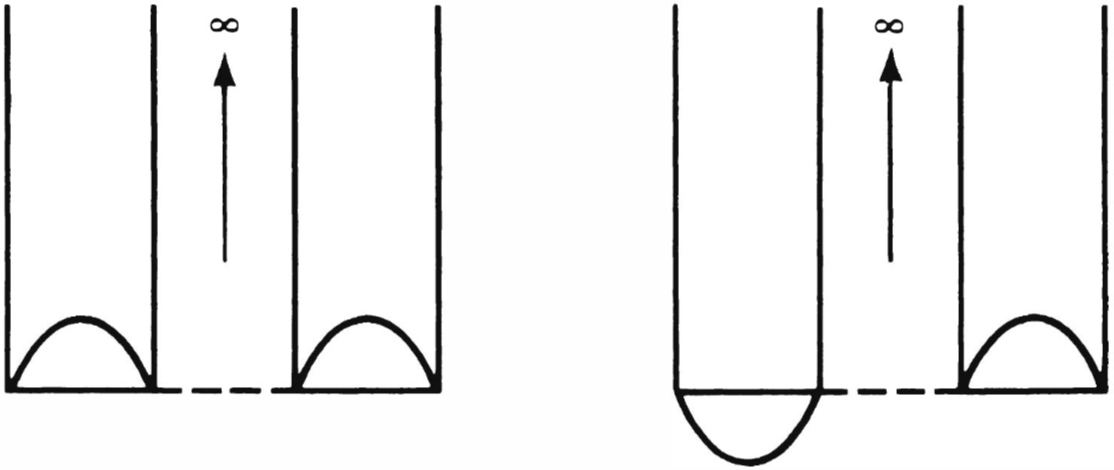
\includegraphics[width=8cm]{Symmetry/infinitedoublewell.png}
\caption{中间势垒趋于无穷高的对称双井}
%\label{default}
\end{center}
\end{figure}

对称双井可用于描述氨分子振荡。氨分子中的N原子可以在三个H原子的上面,也可在三个H原子的下面。N原子和三个H原子组成金字塔,N原子是塔尖,三个H原子构成金字塔的底面。氨分子整体可围绕通过塔尖和底面中心的轴转动,塔尖(N)是否在底面($H_3$)的上面是相对于这个转动而言的。由于氨分子中正、负电荷中心不重合,N端稍带负电,$H_3$端稍带正电,氨分子整体有非零的电偶极矩\index{electric dipole moment:电偶极矩}(electric dipole moment),由N指向$H_3$。

\begin{figure}[htbp]
\begin{center}
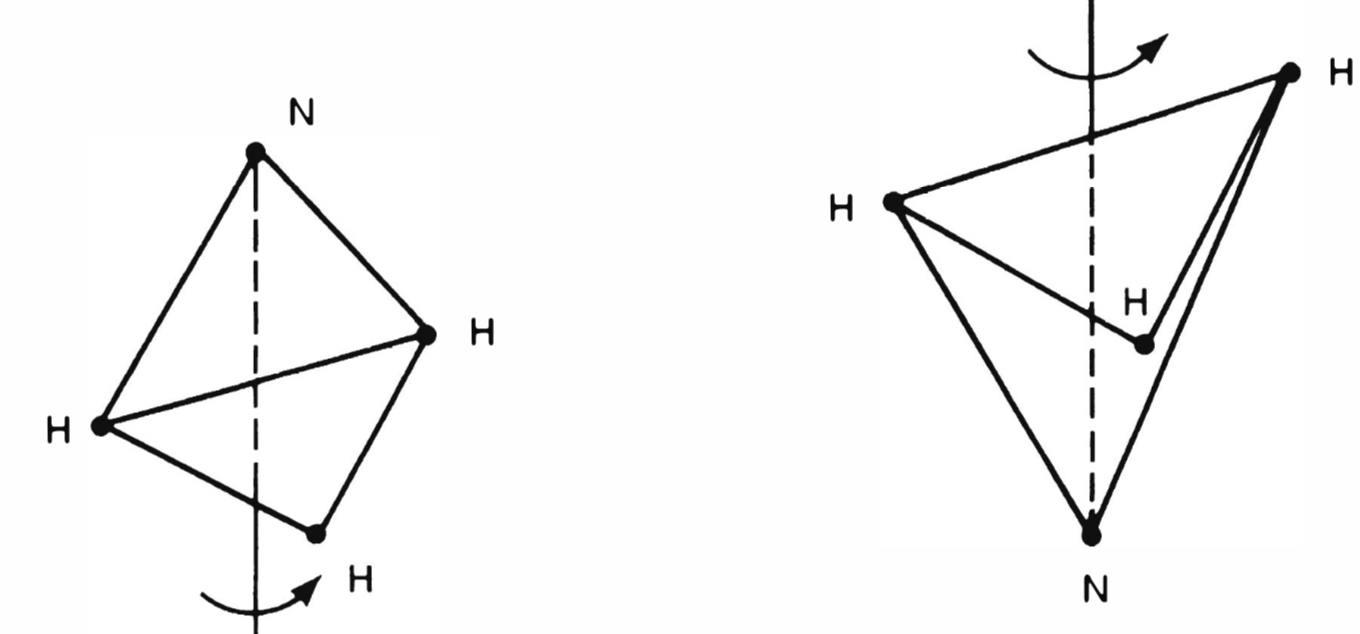
\includegraphics[width=9cm]{Symmetry/amoniamolecule.png}
\caption{氨分子}
%\label{default}
\end{center}
\end{figure}

氨分子对称构型和反对称构型的能量差($\approx  \times 10^{-4} eV$)对应的频率是$24000$MHz,对应波长是1cm。对应电磁波谱中的微波。对$PH_3$而言,它具有和$NH_3$类似的结构,但P比N更难“隧穿”$H_3$平面,频率只有$NH_3$的十分之一。对更重的$PF_3$,我们甚至无法测量到P“隧穿”$F_3$平面的频率。

\subsection*{参考}

J. J. Sakurai, Modern Quantum Mechanics, \S 4.1, 4.2

P. W. Anderson, More is Different, Science, New Series, Vol. 177, No. 4047 (Aug 4, 1972), pp393-396

\section{时间反演对称}

分立的对称性除宇称(P,$x \to -x$)外,还有电荷共轭(C,$q \to -q$,即粒子$\to$反粒子),时间反演(T,$t \to -t$)。在弱相互作用中,单独的C对称,P对称,和联合的CP对称都不存在。必须加上T,联合的CPT对称存在。可以证明,点粒子必须满足联合的CPT对称和洛伦兹协变对称(CPT Theorem)。

本节将主要讨论时间反演对称。

\subsection{运动反演}

首先我们来做个“正名”的工作(所谓“名不正,则言不顺;言不顺,则事不成。”)。说“时间反演”\index{Time reversal:时间反演}(Time reversal)其实并不恰当,它会让人们误以为物理学家在讨论“回到过去”,“时空旅行”等,至少在这里我们所讨论的时间反演与这些是无关的。

就我们这里即将展开的讨论,更确切的名称应该是运动反演\index{reversal of motion:运动反演}(reversal of motion)。比如对经典力学,假设粒子在势场$V(x)$中运动,根据牛顿力学$F = m \ddot x = - \nabla V(x)$,我们求出粒子运动的轨迹$x(t)$。

所谓运动反演就是在某个特定的时刻,比如$t_0$,粒子的运动反向,$v \to - v$或$p \to -p$,我们发现$x(t)$仍然是$F = m \ddot x$的解,粒子运动的轨迹与运动反演前重合。我们称这种变换下的不变性称为运动反演对称,当然按物理学的常规术语,我们称其为时间反演对称。

%这里有一些标准的讨论,比如时间反演就相当于“倒着放”一段电影,在经典力学适用的场景下,只看影像运动,我们是无法断定影片是“正放”还是“倒放”的。这就是所谓时间反演对称。但对存在耗散(dissipation)的物理过程就不一样了,比如一个铅球落在一滩烂泥里,铅球的势能会转变为动能,动能最终会转变为热能,体现为烂泥和铅球温度的上升。对存在耗散的物理过程,熵是单边增大的($\Delta S \ge 0$)。据此我们很容易判别出哪段影片是“倒放”的(非物理的),而哪段影片是“正放”的(物理的)。

%比如我们可以设想一个人坐在玻璃房子里抽烟,最终烟尘将弥漫满整个房间,这是物理的。相反如果我们将此段影像“倒放”,我们将会看到充满整个房间的烟尘都逐渐聚集并“凝结”为一根香烟,这就是非物理的了。

%换句话说在以上过程中“正放”的影像对应一个物理法则(熵增),而“倒放”的影像对应一个非物理的法则(熵减)。

这里我们不讨论存在“耗散”\index{dissipation:耗散}(dissipation)的物理过程,仅指出两点:(1)“耗散”与一段时间有关,比如摩擦的发生总是要经历一段时间的,但时间反演则是发生在$t_0$瞬间的变换。(2)时间反演指的是在某特定时刻$t_0$,构成物理系统所有粒子的运动反演$v_i \to - v_i$或$p_i \to - p_i$(同时$x_i \to x_i$)。这暗示我们对系统信息的全盘和全部的掌握,但热力学的基本假设就是我们不可能具有此等对信息的全盘和全部掌握。由于适用条件的不同,我们不讨论如何把时间反演对称推广至包含耗散的物理过程。

这里我们提出两个任务:(1)如何把时间反演概念推广至电磁学;(2)如何把时间反演概念推广至量子力学。

电磁场的物理规律是麦克斯韦方程组\index{Maxwell equations:麦克斯韦方程组},

\begin{equation}
\nabla \cdot E = 4 \pi \rho, \nabla \times B - \frac{1}{c} \frac{\partial E}{\partial t} = \frac{4 \pi j}{c}, \nabla \times E = - \frac{1}{c} \frac{\partial B}{\partial t}
\end{equation}

带电粒子的运动方程由洛伦兹力\index{Lorentz Force:洛伦兹力}给定,

\begin{equation}
F = e \left( E + \frac{v \times B}{c}   \right)
\end{equation}

时间反演\index{Time reversal:时间反演}$t \to -t$,如果满足:

\begin{equation}
E \to E, B \to -B, \rho \to \rho, j \to -j, v \to -v
\end{equation}

可以验证此时麦克斯韦方程组和洛伦兹力的公式仍然成立。即我们有了某种变换下的不变性,这样我们就把时间反演概念推广到了电磁学的领域。(值得注意的是为了保证麦克斯韦方程组和洛伦兹力的公式不变,$t \to -t$变换的选择并不是唯一的,比如我们可以选择:$E \to -E$, $B \to B$, $\rho \to - \rho$, $j \to j$, $v \to -v$)

把时间反演概念推广到量子力学比较复杂,但有证据表明如果可以的话,时间反演和“取复共轭”这个操作有关。

考虑薛定谔方程(S.E.):

\begin{equation}
i \hbar \frac{\partial \psi}{\partial t} = \left( - \frac{\hbar^2}{2m}\nabla^2 + V \right) \psi
\end{equation}

假设$\psi(x,t) = u_n (x) e^{- i E_n t / \hbar}$是S.E.的解,那么$\psi(x, -t)$不是S.E.的解,但$\psi^* (x, -t)$就又是S.E.的解了。(这里我们假设对时间反演态,比如$\psi^* (x, -t)$,S.E.仍成立,就好像在经典力学中我们发现对$x(-t)$,牛顿方程仍成立。)

\subsection{反幺正算符}

以前我们讨论的种种对称变换都是幺正变换,这意味着当$\left| \alpha \right\rangle \to \left| \tilde{ \alpha }  \right\rangle$,$\left| \beta \right\rangle \to \left| \tilde{ \beta }  \right\rangle$,

\begin{equation}
\left\langle \beta | \alpha \right\rangle \to \left\langle \tilde{\beta} | \tilde{\alpha} \right\rangle = \left\langle \beta \right| U^\dagger U \left| \alpha \right\rangle = \left\langle \beta | \alpha \right\rangle 
\end{equation}

即态矢量的内积在幺正变换下是不变的。对量子力学而言,几率最终对应力学量的取值,几率对应内积的绝对值的平方。受此启发,我们试着把“态矢量的内积不变”这一要求稍稍放松。

\begin{equation}
\left|  \left\langle \tilde{\beta} | \tilde{\alpha} \right\rangle \right| = \left| \left\langle \beta | \alpha \right\rangle  \right|
\end{equation}

这意味着

\begin{equation}
\left\langle \tilde{\beta} | \tilde{\alpha} \right\rangle = \left\langle \beta | \alpha \right\rangle^* = \left\langle \alpha | \beta \right\rangle
\end{equation}

也是一种可能的选择。我们通过定义反幺正算符\index{Antiunitary operator:反幺正算符}$\theta$来兑现这种选择。

\begin{equation}
\left| \alpha \right\rangle \to \left| \tilde{\alpha} \right\rangle = \theta \left| \alpha \right\rangle, \left| \beta \right\rangle \to \left| \tilde{\beta } \right\rangle = \theta \left| \beta \right\rangle
\end{equation}

反幺正算符$\theta$可表示为幺正算符(U)作用于取复共轭算符(K)的形式:

\begin{equation}
\theta = UK
\end{equation}

反幺正算符满足如下性质:

\begin{eqnarray}
\left\langle \tilde{\beta} | \tilde{\alpha} \right\rangle  &  =  &  \left\langle \beta | \alpha \right\rangle^*  \\
\theta \left( c_1 \left| \alpha \right\rangle + c_2 \left| \beta \right\rangle \right) & = & c_1^* \theta \left| \alpha \right\rangle + c_2^* \theta \left| \beta \right\rangle 
\end{eqnarray}

这里需要注意,(2)对基矢$\left| a' \right\rangle$取复共轭仍然是$\left| a' \right\rangle$,

\begin{equation}
K \left| a' \right\rangle = \left| a' \right\rangle
\end{equation}

(2)另外对$\theta$而言,由于它是反幺正、反线性的,在算式中要把它看做是向右侧运算的。(Sakurai:it is always safer to work with the action of $\theta$on kets only. )我们也不试图去定义$\theta$的厄米共轭$\theta^\dagger$。

现在来证明对$\theta = UK$,$\left\langle \tilde{\beta} | \tilde{\alpha} \right\rangle  =  \left\langle \beta | \alpha \right\rangle^* $。

首先,

\begin{equation}
\left| \alpha \right\rangle = \sum\limits_{a'} \left| a' \right\rangle \left\langle a' | \alpha \right\rangle 
\end{equation}

对其施以反幺正变换,

\begin{equation}
\left| \tilde{\alpha} \right\rangle = UK \sum\limits_{a'} \left| a' \right\rangle \left\langle a' | \alpha \right\rangle = \sum\limits_{a'} U \left| a' \right\rangle \left\langle \alpha | a' \right\rangle
\end{equation}

类似地,对$\left| \tilde{\beta} \right\rangle$,

\begin{equation}
\left| \tilde{\beta} \right\rangle = UK \sum\limits_{a''} \left| a'' \right\rangle \left\langle a'' | \beta \right\rangle = \sum\limits_{a''} U \left| a'' \right\rangle \left\langle \beta | a'' \right\rangle
\end{equation}

因此:

\begin{eqnarray*}
\left\langle \tilde{\beta} | \tilde{\alpha} \right\rangle  & = & \sum\limits_{a' a''} \left\langle a'' | \beta \right\rangle \left\langle a'' \right| U^\dagger U \left| a' \right\rangle \left\langle \alpha | a' \right\rangle \\
{}  & = & \sum\limits_{a'} \left\langle \alpha | a' \right\rangle \left\langle a' | \beta \right\rangle = \left\langle \alpha | \beta \right\rangle
\end{eqnarray*}

\subsection{时间反演算符}

首先证明时间反演算符不可能是幺正算符,但可以是反幺正算符\index{Antiunitary operator:反幺正算符}。为了和一般的反幺正算符$\theta$区别开,我们把时间反演算符记为$\Theta$。

\begin{figure}[htbp]
\begin{center}
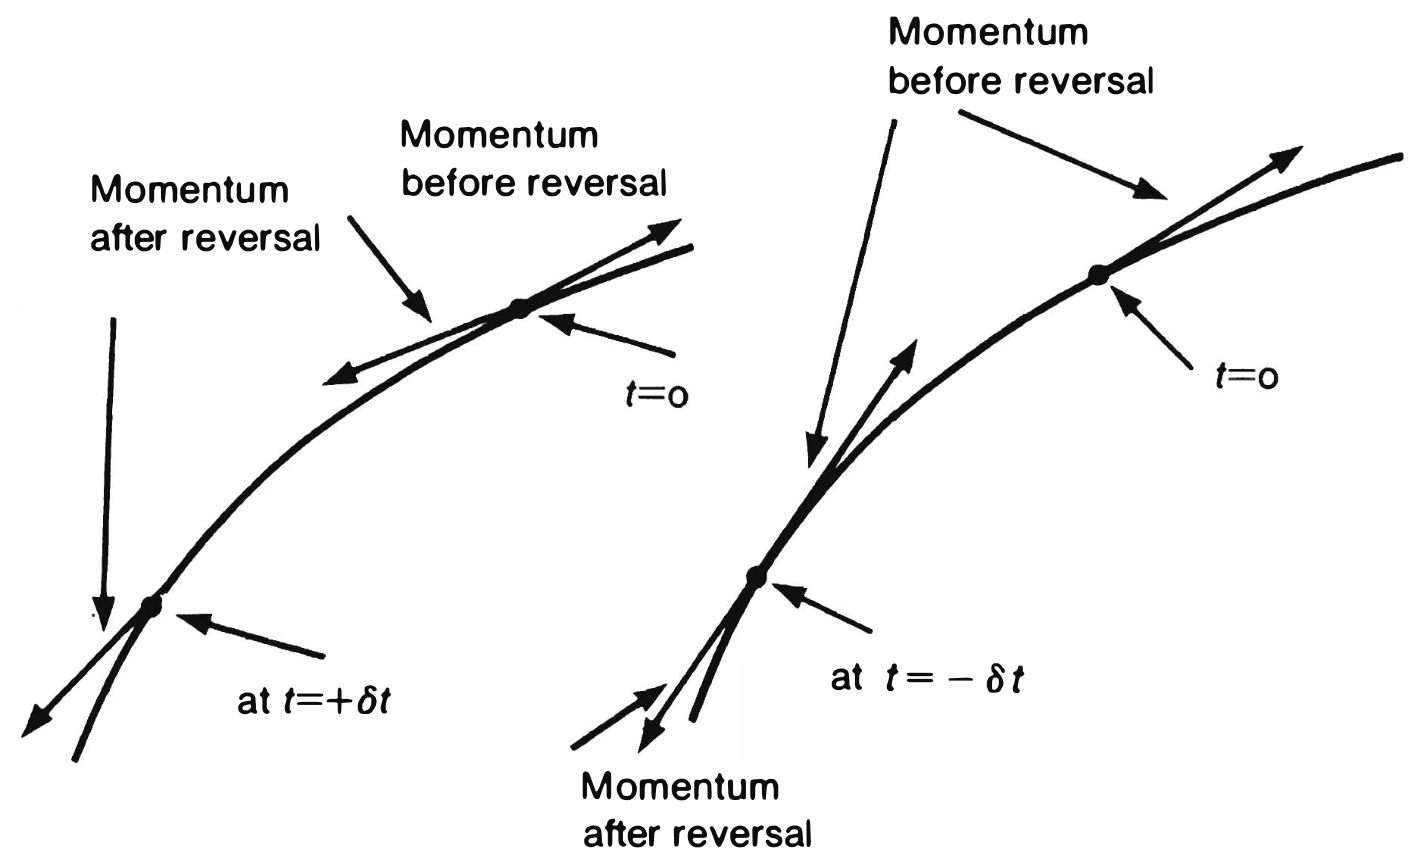
\includegraphics[width=10cm]{Symmetry/timereversal.png}
\caption{$ U(\delta t) \Theta \left| {} \right\rangle = \Theta  U(- \delta t) \left| {} \right\rangle $}
%\label{default}
\end{center}
\end{figure}

我们构造如图两个过程,这两个过程在效果上是相同的。左图对应的是先在$t=0$的时候时间反演\index{Time reversal:时间反演},时间反演后粒子的$p \to -p$,然后再演化$\delta t$,即粒子在$p$的延长线方向上运动$\delta t$时间,对应的量子态是:

\begin{equation}
U(\delta t) \Theta \left| {} \right\rangle
\end{equation}

右图对应的是先让粒子在动量$p$延长线的反方向上退行$\delta t$,然后再时间反演$\Theta$,对应的量子态是:

\begin{equation}
\Theta U(-\delta t) \left| {} \right\rangle  
\end{equation}

$\Theta \left| {} \right\rangle$是$\left| {} \right\rangle$的时间反演态。上述两个量子态相同,意味着:

\begin{equation}
U(\delta t) \Theta \left| {}  \right\rangle = \Theta U(-\delta t) \left| {} \right\rangle
\end{equation}

即:

\begin{equation}
\left( 1 -  \frac{i H \delta t}{\hbar}  \right) \Theta \left| {} \right\rangle = \Theta \left( 1 -  \frac{i H (- \delta t)}{\hbar}  \right) \left| {} \right\rangle
\end{equation}

这意味着:

\begin{equation}
- i H \Theta \left| {} \right\rangle  = \Theta i H \left| {} \right\rangle
\end{equation}

假设$\Theta$是幺正算符,我们可以把等式右侧的$i$直接提到$\Theta$前面去,于是得到:

\begin{equation}
- H \Theta = \Theta H
\end{equation}

但这会导致物理上无法接受的后果。

假设H的能量本征态$\left| n \right\rangle$($H \left| n \right\rangle = E_n \left| n \right\rangle$),

\begin{equation}
H \Theta \left| n \right\rangle = - \Theta H \left| n \right\rangle = - E_n \Theta \left| n \right\rangle
\end{equation}

这意味着$\Theta \left| n \right\rangle$也是H的本征态,且其能量本征值为$- E_n$。我们知道能量的取值是正定的($E \ge 0$),而$- E_n$意味着$E < 0$,这是物理上无法接受的结果。初等物理中喜欢说能量的取值依赖于能量零点的选择,但考虑到$E = m c^2$,能量就是质量,取负的能量意味着取负的质量,而负质量是非物理的,会导致很多奇怪的结果。总之在现有物理学框架内能量是不能小于0的。

假如$\Theta$是反幺正算符\index{Antiunitary operator:反幺正算符},$i$提出到最左边的时候就要加一个负号“-”,这意味着:

\begin{equation}
H \Theta = \Theta H
\end{equation}

对$\left| n \right\rangle$而言,

\begin{equation}
H \Theta \left| n \right\rangle = \Theta H \left| n \right\rangle = E_n \Theta \left| n \right\rangle
\end{equation}

即时间反演态$\Theta \left| n \right\rangle$对应的能量本征值仍是$E_n$,这样就不会导致任何不舒服了。

对宇称\index{Parity:宇称}$\pi$,我们说位置向量$x$在宇称下是奇的

\begin{equation}
\pi x \pi^\dagger = - x
\end{equation}

但这里我们无法定义$\Theta$的厄米共轭,我们使用$\Theta$的逆$\Theta^{-1}$,我们定义

\begin{equation}
\Theta A \Theta^{-1} = \pm A
\end{equation}

这里A是厄米算符,代表某力学量,我们称$\Theta A \Theta^{-1} = A$为时间反演变换下为偶的;而称$\Theta A \Theta^{-1} = - A$为时间反演变换下为奇的。

可以证明对时间反演态$\left| \tilde{\alpha}  \right\rangle$,

\begin{equation}
\left\langle \alpha \right| A \left| \alpha \right\rangle = \left\langle \tilde{\alpha} \right| \Theta A \Theta^{-1} \left| \tilde{\alpha} \right\rangle = \pm \left\langle \tilde{\alpha} \right| A \left| \tilde{\alpha} \right\rangle
\end{equation}

在时间反演下,我们期望动量$p$是奇的,位置$x$是偶的,即:

\begin{eqnarray}
\Theta p \Theta^{-1} & = & - p \\
\Theta x \Theta^{-1} & = & x
\end{eqnarray}

(1)假设$\left| p' \right\rangle$是动量$p$的本征态,那么$\left| p' \right\rangle$的时间反演态$\Theta \left| p' \right\rangle$对应的动量本征值是$- p'$。

动量$p$的本征值问题:

\begin{equation}
p \left| p' \right\rangle = p' \left| p' \right\rangle
\end{equation}

两侧都左乘$\Theta$

\begin{equation}
\Theta p \left| p' \right\rangle = \Theta p \Theta^{-1} \Theta \left| p' \right\rangle = - p \Theta \left| p' \right\rangle = p' \Theta \left| p' \right\rangle
\end{equation}

上式可改写为:

\begin{equation}
p \Theta \left| p' \right\rangle = - p' \Theta \left| p' \right\rangle
\end{equation}

即$\Theta \left| p' \right\rangle$对应的动量本征值为$-p'$。

(2)证明对一般的时间反演态$\Theta \left| {} \right\rangle$,基础对易式\index{fundamental commutation relation:基础对易式}$[x, p] = i \hbar$仍然成立。

首先把算符的等式写完整:

\begin{equation}
[x, p] \left| {} \right\rangle  = i \hbar \left| {} \right\rangle
\end{equation}

两侧都左乘$\Theta$

\begin{equation}
\Theta [x, p] \Theta^{-1} \Theta \left| {} \right\rangle = \Theta i \hbar \left| {} \right\rangle  
\end{equation}

上式可变化为

\begin{equation}
[x, -p] \Theta \left| {} \right\rangle = - i \hbar \Theta \left| {} \right\rangle
\end{equation}

即

\begin{equation}
[x, p] \Theta \left| {} \right\rangle = i \hbar \Theta \left| {} \right\rangle
\end{equation}

(3)假设$\Theta J \Theta^{-1} = -J$,我们可推出角动量的对易关系$[ J_x, J_y ] = i \hbar J_z $

首先:

\begin{equation}
[ J_x, J_y ] \left| {} \right\rangle = i \hbar J_z \left| {} \right\rangle
\end{equation}

两侧左乘$\Theta$

\begin{equation}
\Theta [ J_x, J_y ] \Theta^{-1} \Theta \left| {} \right\rangle = \Theta i \hbar J_z \left| {} \right\rangle
\end{equation}

上式可变化为

\begin{equation}
[ -J_x, -J_y  ] \Theta \left| {} \right\rangle = - i \hbar \Theta J_z \Theta^{-1} \Theta \left| {} \right\rangle
\end{equation}

化简后可得:

\begin{equation}
[J_x, J_y] \Theta \left| {} \right\rangle = i \hbar J_z \Theta \left| {} \right\rangle
\end{equation}

\subsection{自旋1/2的时间反演}

考察一个任意的自旋1/2的量子态——$\hat n$方向上取“+”的态——$\hat n$的取向用倾角$\beta$和方位角$\alpha$表示:

\begin{equation}
\left| n, + \right\rangle = e^{-i S_z \alpha / \hbar } e^{- i S_y \beta / \hbar} \left| + \right\rangle
\end{equation}

即通过对$\left| + \right\rangle$先围绕y轴转$\beta$再围绕z轴转$\alpha$来得到$\left| n, + \right\rangle$的量子态。

$\left| n, + \right\rangle$的时间反演态对应的是在$\hat n$方向上取“-”的量子态,考虑到相位的不确定,我们把它表示为:

\begin{equation}
\Theta \left| n, + \right\rangle = \eta  \left| n, - \right\rangle
\end{equation}

上式左侧可表示为:

\begin{eqnarray*}
\Theta \left| n, + \right\rangle  & = & \Theta e^{-i S_z \alpha / \hbar } e^{- i S_y \beta / \hbar} \left| + \right\rangle \\
{} & = & \Theta e^{-i S_z \alpha / \hbar } \Theta^{-1} \Theta e^{- i S_y \beta / \hbar} \Theta^{-1} \Theta \left| + \right\rangle \\
{} & = & e^{-i S_z \alpha / \hbar } e^{- i S_y \beta / \hbar}  \Theta \left| + \right\rangle
\end{eqnarray*}

因此:

\begin{equation}
e^{-i S_z \alpha / \hbar } e^{- i S_y \beta / \hbar}  \Theta \left| + \right\rangle = \eta e^{-i S_z \alpha / \hbar } e^{- i S_y (\beta + \pi) / \hbar} \left| + \right\rangle
\end{equation}

这意味着:

\begin{equation}
\Theta = \eta e^{- i S_y \pi / \hbar} K
\end{equation}

上式最后的K是必须放上去的,否则剩余部分就是个幺正算符了,这不符合时间反演算符是反幺正的这一性质。

利用:

\begin{equation}
e^{-i S_y \pi / \hbar } = - i \frac{2S_y}{\hbar}
\end{equation}

这样,我们求出对自旋1/2时间反演算符可表示为

\begin{equation}
\Theta = - i \eta \left( \frac{2 S_y}{ \hbar} \right) K = \eta K \left( \begin{array}{cc} 0 & -1  \\ 1 & 0 \end{array} \right) 
\end{equation}

下面,我们来证明对自旋1/2,有:$\Theta^2 = -1$。

考虑任意态矢量:

\begin{equation}
\chi = \left( \begin{array}{c} c_+  \\  c_- \end{array} \right)
\end{equation}

左乘$\Theta$

\begin{equation}
\Theta \chi = \eta K \left(  \begin{array}{c}  -c_-  \\ c_+  \end{array}  \right) =  \left(  \begin{array}{c}  - \eta c_-^*  \\  \eta c_+^*  \end{array}  \right)
\end{equation}

继续左乘$\Theta$

\begin{equation}
\Theta^2 \chi = \eta K \left(  \begin{array}{c} -\eta c_+^*  \\ - \eta c_-^* \end{array}  \right) = - \eta \eta^* \left( \begin{array}{c} c_+  \\  c_- \end{array} \right) = - \chi
\end{equation}

因此,

\begin{equation}
\Theta^2 = -1
\end{equation}

更一般地,我们能证明对角动量量子数j为半整数,$\Theta^2 = -1$,但对整数的j,$\Theta^2 = 1$(J. J. Sakurai, pp 278-279)。

\subsection{Kramers简并}

由$H \Theta = \Theta H$出发,由于$\Theta$是反幺正、反线性算符,所以我们无法从$H \Theta = \Theta H$得到一个守恒量。但由此式出发,我们可得到Kramers简并的概念。

假设$\left| n \right\rangle$是H的本征态,对应本征值是$E_n$,那么$\left| n \right\rangle$的时间反演态$\Theta \left| n \right\rangle$也是H的本征态,且对应本征值也是$E_n$。

假设对能级$E_n$不存在简并,即$\left| n \right\rangle$和$\Theta \left| n \right\rangle$本质上是一个量子态,二者间只差一个相位$\eta$,

\begin{equation}
\Theta \left| n \right\rangle = \eta \left| n \right\rangle
\end{equation}

这意味着:

\begin{equation}
\Theta^2 \left| n \right\rangle = \Theta \eta \left| n \right\rangle = \eta^* \eta \left| n \right\rangle = \left| n \right\rangle
\end{equation}

即$\Theta^2 =1 $,但我们知道对电子而言,自旋是1/2,这意味着$\Theta^2 $其实是$-1$。这说明时间反演态$\Theta \left| n \right\rangle $和$\left| n \right\rangle$是本质上不同的两个态,即$E_n$存在简并,我们称这种因时间反演不变导致的简并为Kramers简并\index{Kramers degeneracy:Kramers简并}。

容易证明对奇数个电子组成的系统存在Kramers简并,而对偶数个电子组成的系统不存在Kramers简并。外加磁场可将Kramers简并打开。

\subsection*{参考}

J. J. Sakurai, Modern Quantum Mechanics, \S 4.4

\section{相互作用绘景}

\subsection{相互作用绘景}

考虑含时的哈密顿,形式上分为两部分,和时间有关的部分归于相互作用$V(t)$

\begin{equation}
H = H_0 + V(t)
\end{equation}

假设$H_0$的本征值问题已知,

\begin{equation}
H_0 \left| n \right\rangle = E_n \left| n \right\rangle
\end{equation}

在$H_0$表象下,假设$t = 0$,系统处于$\left| i \right\rangle$的态,由于$\left| i \right\rangle$是$H_0$的本征态,而非$H$的本征态,并且$V(t) \neq 0$,我们研究的不再是定态(stationary state),随着时间的演化,那些$n \neq i$的量子态也可能被占据。

假设量子态$\left| \alpha \right\rangle$,用$H_0$表象展开:

\begin{equation}
\left| \alpha \right\rangle = \sum\limits_n  \left| n \right\rangle \left\langle n | \alpha \right\rangle
\end{equation}

$t = 0$时,

\begin{equation}
\left| \alpha \right\rangle = \sum\limits_n c_n(0) \left| n \right\rangle
\end{equation}

$t > 0$时,

\begin{equation}
\left| \alpha, t \right\rangle = \sum\limits_n c_n(t) e^{- i E_n t / \hbar} \left| n \right\rangle
\end{equation}

这里$e^{- i E_n t / \hbar}$是$H_0$导致的,我们能否得到一种形式使$c_n (t)$只由相互作用$V(t)$决定。

%\subsection{相互作用绘景}

考虑变换:

\begin{eqnarray}
\left| \alpha, t \right\rangle_I & = & e^{i H_0 t /\hbar}  \left| \alpha, t \right\rangle_S\\
V_I(t) & = & e^{i H_0 t /\hbar} V_S(t) e^{ - i H_0 t /\hbar}
\end{eqnarray}

这里脚标$I$表示相互作用绘景\index{Interaction Picture:相互作用绘景},$S$表示薛定谔绘景。

对某力学量A,

\begin{equation}
\left\langle A \right\rangle = {}_S\left\langle \alpha,t \right| e^{ - i H_0 t /\hbar} e^{i H_0 t /\hbar} A_S e^{ - i H_0 t /\hbar}   e^{i H_0 t /\hbar} \left| \alpha, t \right\rangle_S
\end{equation}

即:

\begin{equation}
\left\langle A \right\rangle = {}_S\left\langle \alpha, t \right| A_S \left| \alpha, t  \right\rangle_S = {}_I\left\langle \alpha, t \right| A_I \left| \alpha,t  \right\rangle_I
\end{equation}

容易证明:

\begin{eqnarray}
i \hbar \frac{\partial }{\partial t} \left| \alpha,t  \right\rangle_I & = & V_I(t) \left| \alpha,t  \right\rangle_I \\
i \hbar \frac{d A_I}{dt}& = & [A_I(t) , H_0 ]
\end{eqnarray}

即在相互作用绘景下,态矢量$\left| \alpha,t  \right\rangle_I$随时间的演化将完全由相互作用$V_I(t)$决定,而算符$A_I(t)$随时间的演化将只由$H_0$决定。

\subsection{拉比公式}

考虑

\begin{equation}
i \hbar \frac{\partial }{\partial t} \left| \alpha,t  \right\rangle_I = V_I(t) \left| \alpha,t  \right\rangle_I
\end{equation}

左乘$\left\langle n \right|$,

\begin{equation}
i \hbar \frac{\partial }{\partial t}  \left\langle n  | \alpha,t  \right\rangle_I = \sum\limits_m \left\langle n \right| V_I(t) \left| m \right\rangle \left\langle m | \alpha,t  \right\rangle_I
\end{equation}

这里

\begin{eqnarray*}
\left\langle n \right| V_I(t) \left| m \right\rangle & = & \left\langle n \right| e^{iH_0t / \hbar} V e^{-iH_0t / \hbar} \left| m \right\rangle  \\
 {} & = & \left\langle n \right| V \left| m \right\rangle e^{i(E_n - E_m)t / \hbar} \\
{} & = & V_{nm} e^{i(E_n - E_m)t / \hbar}
\end{eqnarray*}

即

\begin{equation}
i \hbar \frac{\partial }{\partial t} c_n(t) = \sum\limits_m V_{nm} e^{i \omega_{nm} t} c_m(t)
\end{equation}

这里:$E_n - E_m = \hbar \omega_{nm}$。

考虑双态系统:

\begin{equation}
H = H_0 + V(t) = \left( \begin{array}{cc} E_1 & \gamma e^{i \omega t} \\  \gamma e^{- i \omega t} & E_2  \end{array} \right)
\end{equation}

假设$t=0$时,$c_1 (0) = 1$,$c_2 (0) = 0$,即粒子全部位于“1”态。可求出$t$时,粒子位于“2”态的几率是:

\begin{equation}
|c_2(t)|^2 = \frac{\gamma^2 / \hbar^2}{\gamma^2 / \hbar^2 + (\omega - \omega_{21})^2 / 4} \sin^2 \left[ t \sqrt{ \frac{\gamma^2}{\hbar^2} + \frac{(\omega - \omega_{21})^2}{4} }    \right]
\label{Rabi's formula}
\end{equation}

其中:$\omega_{21} = \frac{E_2 - E_1}{\hbar}$。公式[\ref{Rabi's formula}]即所谓拉比公式(Rabi's formula)。

\subsection{戴逊级数}

定义相互作用绘景下的演化算符$U_I(t, t_0)$,

\begin{equation}
\left| \alpha,t  \right\rangle_I = U_I(t, t_0) \left| \alpha,t_0 \right\rangle_I
\end{equation}

$U_I(t, t_0)$遵从如下微分方程:

\begin{equation}
i \hbar \frac{d}{dt } U_I (t, t_0) = V_I (t) U_I(t, t_0)
\end{equation}

假设初始条件:$U_I(t, t_0)|_{t = t_0} = 1$

迭代一次,解出$U_I(t, t_0)$,

\begin{equation}
U_I(t, t_0) = 1 - \frac{i}{\hbar} \int_{t_0}^t dt' V_I(t') U_I (t', t_0) 
\end{equation}

反复迭代,

\begin{eqnarray*}
U_I(t, t_0) & = & 1 - \frac{i}{\hbar}\int_{t_0}^t dt' V_I(t') +  \\
{} & {} & \left(\frac{-i}{\hbar} \right)^2 \int_{t_0}^t dt' \int_{t_0}^{t'} dt'' V_I (t') V_I(t'') + ... +  \\
{} & {} &  \left(\frac{-i}{\hbar} \right)^n \int_{t_0}^t dt' \int_{t_0}^{t'} dt'' ... \int_{t_0}^{t^{(n-1)}} dt^{(n)} V_I(t') V_I (t'')... V_I(t^{(n)}) \\
{} &  {}  & + ... 
\end{eqnarray*}

这就是所谓戴逊级数\index{Dyson Series:戴逊级数}(Dyson series)。

由于不同时刻的$V_I$不一定是对易的,我们必须保证积分号里$V_I(t') V_I (t'')... V_I(t^{(n)}$各个时间的次序满足$t > t' > t'' > ... > t^{(n-1)} > t^{(n)} >... > t_0$。

\subsection*{参考}

J. J. Sakurai, Modern Quantum Mechanics, \S 5.5, 5.6

\section{散射的形式理论}

考虑不含时的量子力学问题

\begin{equation}
H = H_0 + V
\end{equation}

假设$H_0$是自由的运动,

\begin{equation}
H_0 = \frac{p^2}{2m}
\end{equation}

其解记为

\begin{equation}
H_0 \left| \phi \right\rangle = E \left| \phi \right\rangle
\end{equation}

$H_0$对应的是入射粒子距离散射中心很远,或粒子被散射改变运动方向后又飞到距离散射中心很远的情形。两种情况$V$都可忽略不计。$H_0$的解可以是单色平面波\index{plane wave:平面波}(plane wave, $\left| p' \right\rangle$)或球面波\index{spherical wave:球面波}(spherical wave, $\left| klm \right\rangle$)。

在球坐标系下,我们可以证明

\begin{equation}
H_0 = - \frac{\hbar^2}{ 2m }  \frac{1}{r^2} \frac{\partial }{\partial r} r^2 \frac{\partial }{\partial r}  + \frac{L^2}{ 2m r^2}
\end{equation}

这里$L^2$是角动量算符的平方。本证函数可以按$R_{El} Y_{lm}$的方式分离变量,矢径部分:

\begin{equation}
- \frac{\hbar^2}{ 2m } \left( \frac{1}{r^2} \frac{\partial }{\partial r} r^2 \frac{\partial }{\partial r} - \frac{l (l + 1)}{ r^2}  \right) R_{El} = E R_{El}
\end{equation}

以上微分方程在变量变换

\begin{equation}
R_{El} = \frac{\chi_{El}}{r}
\end{equation}

下大大简化:

\begin{equation}
\chi'' + \left( \frac{2mE}{\hbar^2} - \frac{l(l+1)}{r^2} \right) \chi = 0
\end{equation}

当散射粒子远离散射中心时,$\frac{l(l+1)}{r^2}$项可忽略不计,同时考虑$E = \hbar^2 k^2 /2m$,微分方程变为:

\begin{equation}
\chi'' + k^2 \chi = 0
\end{equation}

它的解为:$e^{\pm i kr}$,再考虑到$R = \chi / r$,矢径部分的波函数为:

\begin{equation}
R_{El} (r) = \frac{e^{\pm i kr} }{r}
\end{equation}

我们可以把散射想象为三个区域:(1)粒子由无穷远入射,假设在$\hat z$方向上,波函数$\sim e^{i kz}$。(2)粒子在散射中心附近,$V$必须考虑,$H = H_0 +V $的本征值问题我们下面会展开讨论。(3)粒子被散射到无穷远去,如果只考虑弹性散射的话,波矢$k$的方向会改变,但大小不会变,此时哈密顿量为$H_0$,波函数$\sim \frac{e^{ikr}}{r} f( \theta, \phi )$。这里$\theta $和$\phi$是用来表示入射的$k \hat z$与散射的$k$的交角\footnote{在本笔记中我尽量不使用矢量的记号,主要目的是为了使公式看起来更简洁,如果你懂的话,自然会知道哪个字母表示的是矢量,哪个不是。}。

\subsection{李普曼-施温格方程}

假设散射是弹性的,$H_0 + V$也具有连续的能谱,并且本征值问题

\begin{equation}
( H_0 + V ) \left| \psi \right\rangle = E \left| \psi \right\rangle
\end{equation}

对应的E和$H_0 \left| \phi \right\rangle = E \left| \phi \right\rangle$对应的E是一样的。当$V \to 0$时,$\left| \psi \right\rangle \to \left| \phi \right\rangle$。

在形式上我们把$\left| \psi \right\rangle$记为:

\begin{equation}
\left| \psi \right\rangle = \frac{1}{E - H_0} V \left| \psi \right\rangle + \left| \phi \right\rangle
\end{equation}

对上式而言,(1)满足$V \to 0$,$\left| \psi \right\rangle \to \left| \phi \right\rangle$。(2)对$V \neq 0$,

\begin{equation}
(E - H_0 - V) \left| \psi \right\rangle = ( E - H_0 ) \left| \phi \right\rangle
\end{equation}

即

\begin{equation}
( E - H_0 ) \left| \psi \right\rangle = V \left| \psi \right\rangle + ( E - H_0 ) \left| \phi \right\rangle
\end{equation}

等式左右都左乘$( E - H_0)^{-1} $

\begin{equation}
\left| \psi \right\rangle = ( E - H_0)^{-1} V \left| \psi \right\rangle + \left| \phi \right\rangle
\end{equation}

为了保证算符$( E - H_0)^{-1} $有意义,将其改写为$\frac{1}{E - H_0 \pm i \epsilon}$,对应把$E$的定义由实数轴延拓到复数域上。

\begin{equation}
\left| \psi^{(\pm)} \right\rangle = \left| \phi \right\rangle + \frac{1}{E - H_0 \pm i \epsilon } V \left| \psi^{(\pm)} \right\rangle
\end{equation}

上式即所谓“李普曼-施温格方程”\index{Lippmann-Schwinger equation:李普曼-施温格方程}(Lippmann-Schwinger equation)。$\left| \psi^{(\pm)} \right\rangle$和“$\pm i \epsilon$”对应。

位置表象,

\begin{equation}
\left\langle x | \psi^{(\pm)} \right\rangle = \left\langle x | \phi \right\rangle + \int d^3 x' \left\langle x \right| \frac{1}{E- H_0 \pm i \epsilon} \left| x' \right\rangle \left\langle x' \right| V \left| \psi^{(\pm)} \right\rangle   
\end{equation}

对上式,定义积分的“核”是,

\begin{equation}
G_{\pm} (x, x') = \frac{\hbar^2}{2m} \left\langle x \right| \frac{1}{E- H_0 \pm i \epsilon} \left| x' \right\rangle
\end{equation}

可以证明:

\begin{equation}
G_{\pm} (x, x') = - \frac{1}{4 \pi} \frac{e^{\pm i k |x - x'|}}{|x - x'|}
\end{equation}

考虑$\left| \phi \right\rangle$是单色平面波,首先换到动量表象,

\begin{equation}
\left\langle x \right| \frac{1}{...}  \left| x' \right\rangle = \frac{\hbar^2}{2m} \int d^3 p' \int d^3 p'' \left\langle x | p' \right\rangle \left\langle p' \right| \frac{1}{E - \frac{p'^2 }{2m } \pm i \epsilon} \left| p'' \right\rangle \left\langle p'' | x' \right\rangle
\end{equation}

其中

\begin{equation}
\left\langle p' \right| \frac{1}{E - \frac{p'^2 }{2m } \pm i \epsilon} \left| p'' \right\rangle = \frac{ \delta^3 (p' - p'')  }{E - \frac{p'^2 }{2m } \pm i \epsilon}
\end{equation}

考虑单色平面波的表达式

\begin{equation}
\left\langle x | p' \right\rangle = \frac{e^{i p' \cdot x / \hbar }}{ (2 \pi \hbar)^{3/2}}
\end{equation}

现在积分变为

\begin{equation}
\frac{\hbar^2}{2m } \int \frac{d^3 p'}{( 2 \pi \hbar)^3} \frac{e^{i p' \cdot (x- x') / \hbar}}{E - \frac{p'^2 }{2m } \pm i \epsilon}
\end{equation}

选向量$x - x'$方向为极轴方向建立球坐标系,令$p' = \hbar q$,波矢$q$方向与$x - x'$方向的夹角为倾角$\theta$。$d^3 p' = \hbar^3 d^3 q = \hbar^3 q^2 dq \sin \theta d \theta d \phi $。积分限:

\begin{eqnarray*}
q & : & 0 \to \infty \\
\theta & : & 0 \to \pi \\
\phi & : & 0 \to 2 \pi
\end{eqnarray*}

变量变换:$\sin \theta d \theta = - d \cos \theta$, $ t = \cos \theta$

\begin{equation}
\frac{1}{(2 \pi)^3} \int_0^{\infty} q^2 dq \int_0^{2 \pi} d \phi \int_{-1}^1 \frac{d t  e^{i q |x - x'| t}}{k^2 - q^2 \pm i \epsilon} 
\end{equation}

这里假设$E = \frac{\hbar^2 k^2}{ 2m }$

\begin{eqnarray*}
I & = & \frac{1}{4 \pi^2}  \frac{1}{i | x-x' |} \int_0^{\infty} q dq \frac{ e^{i q |x-x'|} - e^{ - i q |x-x'|} }{k^2 - q^2 \pm i \epsilon }  \\
{} & = &  \frac{-1}{4 \pi^2} \frac{1}{i | x-x' |} \int_0^{\infty} q dq \frac{ e^{i q |x-x'|  }  - e^{-i q |x-x'|} }{ q^2 - k^2  \mp i \epsilon }  \\
{} & = & \frac{i}{4 \pi^2 | x-x' | }  \int_{- \infty}^{\infty} \frac{q dq e^{i q |x - x'|}}{ q^2 - k^2 \mp i \epsilon }
\end{eqnarray*}

考虑

\begin{equation}
\frac{1}{q - k \mp i\epsilon' } + \frac{1}{q + k \pm i \epsilon' } = \frac{2 q}{q^2 - k^2 \mp i \epsilon }
\end{equation}

\begin{figure}[htbp]
\begin{center}
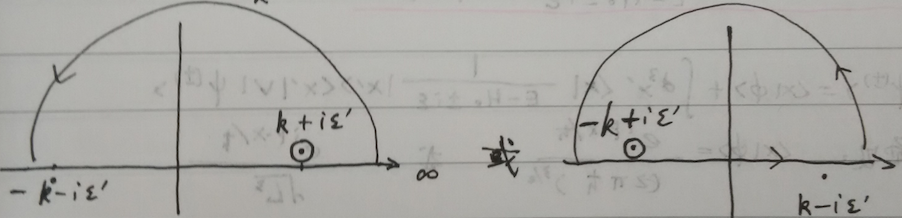
\includegraphics[width=10cm]{Scattering/TheContour.png}
\caption{奇点位置和积分回路。}
%\label{default}
\end{center}
\end{figure}


对“upper sign”,奇点位置:

\begin{equation}
q = k + i \epsilon' , q= - k - i \epsilon' 
\end{equation}

对“lower sign”,奇点位置:

\begin{equation}
q = k - i \epsilon' , q= - k + i \epsilon' 
\end{equation}

由于被积函数中出现的是$e^{i q |x - x'|}$,积分回路选上半回路(即$q: - \infty \to \infty$,然后上半回路绕回$q \to - \infty$)。对“upper sign”,回路绕过奇点:$q = k + i \epsilon'$,对“lower sign”,回路绕过奇点:$q= - k + i \epsilon'$。

根据留数定理\index{Residue theorem:留数定理}:

\begin{equation}
I = \frac{i}{4 \pi^2 }\frac{2 \pi i}{2} \frac{e^{ \pm i k |x-x'|}}{|x-x'|}  = - \frac{1}{4 \pi} \frac{e^{ \pm i k |x-x'|}}{|x-x'|}
\end{equation}

即

\begin{equation}
G_{\pm} (x, x') = - \frac{1}{4 \pi} \frac{e^{\pm i k |x - x'|}}{|x - x'|}
\end{equation}

因此

\begin{equation}
\left\langle x | \psi^{(\pm)} \right\rangle = \left\langle x | \phi \right\rangle - \frac{2m}{\hbar^2} \int d^3 x' \frac{e^{\pm i k |x-x'|}}{4 \pi |x-x'| } \left\langle x' \right| V \left| \psi^{(\pm)} \right\rangle 
\end{equation}

上式说明(特定能量)不含时弹性散射的解相当于“单色平面波”\index{plane wave:平面波}($\left\langle x | \phi \right\rangle$)加上一个向外或向内传播的球面波\index{spherical wave:球面波}($\frac{e^{\pm i k  r}}{r }$)。

其中

\begin{equation}
\left\langle x' \right| V \left| \psi^{(\pm)} \right\rangle = \int d^3 x'' \left\langle x' \right| V \left| x'' \right\rangle \left\langle x'' | \psi^{(\pm)} \right\rangle
\end{equation}

假设V是局域(local)的。即$V(x')$只和位置$x'$有关。

\begin{equation}
\left\langle x' \right| V \left| x'' \right\rangle = V(x' ) \delta^3 (x' -x'')
\end{equation}

则

\begin{equation}
\left\langle x' \right| V \left| \psi^{(\pm)} \right\rangle = V(x') \left\langle x' | \psi^{(\pm)} \right\rangle
\end{equation}

现在:

\begin{equation}
\left\langle x | \psi^{(\pm)} \right\rangle = \left\langle x | \phi \right\rangle - \frac{2m}{\hbar^2} \int d^3 x' \frac{e^{\pm i k |x-x'|}}{4 \pi |x-x'| } V(x') \left\langle x' | \psi^{(\pm)} \right\rangle 
\end{equation}

这里$x'$是“源点”,对应$V(x')$,我们要对所有源点积分得到“场点”$x$处的波函数$\left\langle x | \psi^{(\pm)} \right\rangle$。

\subsection{微分散射截面}

散射问题通常关心的是“远场”,

\begin{equation}
|x| >> |x'|
\end{equation}

散射发生在空间有限狭小区域内,而我们在远离相互作用$V(x')$的“场点”$x$观察粒子在空间取向上的分布,如果入射波函数的波矢是$k$,散射波函数的波矢是$k'$,那么就是散射波函数的模方与“$k'$和$k$之间夹角”$( \theta, \phi$ )的关系。这个关系包含了相互作用$V(x')$的信息。(比如原子核的大小只有$10^{-15}$米,但我们通过研究散射可推知原子核的内部结构与相互作用。)

\begin{figure}[htbp]
\begin{center}
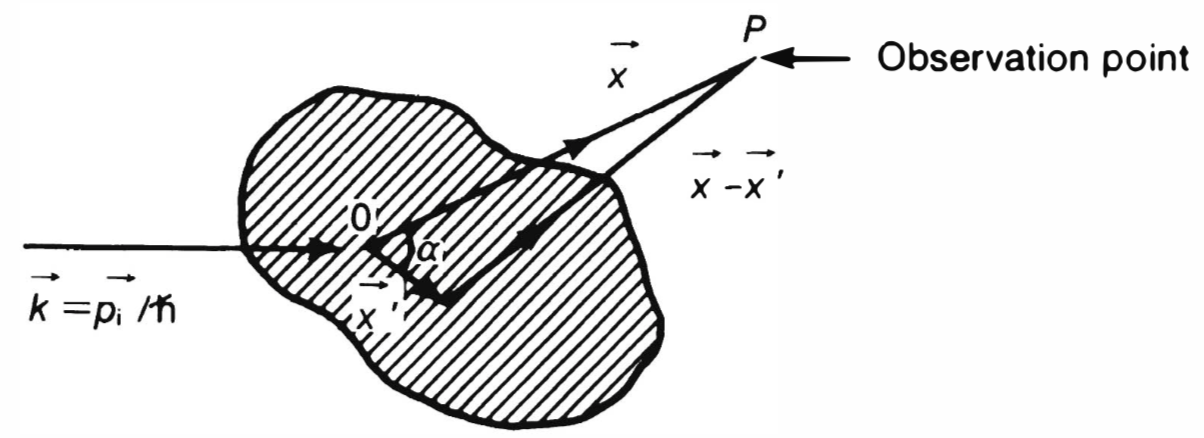
\includegraphics[width=10cm]{Scattering/sourcefields.png}
\caption{我们在场点$x$观察粒子的散射,而散射发生的区域则局限在源点$x'$。}
%\label{default}
\end{center}
\end{figure}

在远场条件下,

\begin{eqnarray*}
|x-x' |  & = & \sqrt{ r^2 + r'^2 - 2 r r' \cos \alpha }  \\ 
{} & = & r \sqrt{ 1- \frac{2r'}{r} \cos \alpha + \frac{r'^2}{r^2 } } \\
{} & \approx & r- \hat r \cdot x'
\end{eqnarray*}

这里

\begin{equation}
\hat r = \frac{x}{|x|}
\end{equation}

出射波函数波矢

\begin{equation}
k' = k \hat r
\end{equation}

这样

\begin{equation}
e^{\pm i k |x-x'| } \approx e^{\pm i k r} e^{\mp i k' \cdot x'}
\end{equation}

这里$k'$表示散射后的波矢,它的方向在空间某个$( \theta, \phi )$的取向上。由于弹性散射,它的大小还是$k$,$k'$的方向与矢径$r$的方向相同,对应$e^{i k r}$。

在远场条件下,出射波函数$\psi^{(+)}$为,

\begin{equation}
\left\langle x | \psi^{(+)}\right\rangle = \left\langle x | k \right\rangle - \frac{1}{4 \pi} \frac{2m}{\hbar^2} \frac{e^{i k r}}{r} \int d^3 x' e^{- i k' \cdot x' } V(x') \left\langle x' | \psi^{(+)}\right\rangle
\label{OutgoingWaveFunction}
\end{equation}

定义

\begin{eqnarray*}
f(k',k) & = & \frac{1}{4 \pi} \frac{2m}{\hbar^2} (2\pi)^3 \int d^3 x' \frac{e^{-i k' \cdot x'}}{(2 \pi)^{3/2}} V(x') \left\langle x' | \psi^{(+)} \right\rangle \\
{} & = & - \frac{1}{4\pi}(2 \pi)^3 \frac{2m}{ \hbar^2 } \left\langle k' \right| V \left| \psi^{(+)} \right\rangle
\end{eqnarray*}

假设入射波在$\hat z$方向上,$\psi^{(+)} (x)$现在可写为:

\begin{equation}
\psi^{(+)} (x) = \frac{1}{(2 \pi)^{3/2}} \left[ e^{i k z} + \frac{e^{ikr}}{r} f(k', k)  \right]
\end{equation}

对上式,我们可分别计算入射几率流$j_i$和散射几率流$j_s$:

\begin{eqnarray}
j_i & = & \frac{\hbar k}{m} \\
j_s & = & \frac{\hbar k}{m} \frac{|f(k', k)|^2}{r^2}
\end{eqnarray}

散射粒子数$dn$

\begin{equation}
d n = j_s r^2 d \Omega
\end{equation}

应正比于入射流$j_i$,立体角微元$d \Omega$和微分散射截面\index{Differential cross-section:微分散射截面}$\sigma_c = \frac{d \sigma}{d \Omega}$。

\begin{equation}
d n = \sigma_c j_i d \Omega
\end{equation}

因此,

\begin{equation}
\sigma_c = \frac{d \sigma}{d \Omega} = \frac{d n}{ j_i d \Omega  }=\frac{ j_s r^2 d \Omega }{j_i d \Omega} = |f(k',k)|^2
\end{equation}

所谓一阶的玻恩近似\index{Born Approximation:玻恩近似}就是直接用$\left| k \right\rangle$代替公式[\ref{OutgoingWaveFunction}]右侧的$\left| \psi^{(+)} \right\rangle$ 。

\subsection{高阶玻恩近似}

把公式[\ref{OutgoingWaveFunction}]右侧的$V \left| \psi^{(+)} \right\rangle$形式地改写为:

\begin{equation}
V \left| \psi^{(+)} \right\rangle = T \left| \phi \right\rangle 
\end{equation}

考虑到李普曼-施温格方程,

\begin{equation}
V \left| \psi^{(+)} \right\rangle = V \left| \phi \right\rangle + V \frac{1}{E- H_0 + i \epsilon} T \left| \phi \right\rangle = T \left| \phi \right\rangle
\end{equation}

这意味着

\begin{equation}
T = V + V \frac{1}{E - H_0 + i \epsilon} T
\end{equation}

散射振幅$f(k',k)$可写为,

\begin{equation}
f(k',k) = - \frac{1}{4 \pi} \frac{2m}{\hbar^2} (2\pi)^3 \left\langle k' \right| T \left| k \right\rangle
\end{equation}

变换矩阵可以一直迭代下去:

\begin{equation}
T = V + V \frac{1}{E - H_0 + i \epsilon} V + V \frac{1}{E - H_0 + i \epsilon} V \frac{1}{E - H_0 + i \epsilon} V + ...
\end{equation}

相互作用$V$出现几次,就是几阶玻恩近似。

\subsection{光学定理}

\begin{equation}
\Im f(\theta = 0) = \frac{k \sigma_t}{4 \pi}
\end{equation}

这里$\theta =0$表示向前散射\index{forward scattering:向前散射}(forward scattering),$k' = k$。$\sigma_t$表示总散射截面(即空间各取向微分散射截面的总和)

\begin{equation}
\sigma_t = \int \frac{d \sigma }{d \Omega} d \Omega
\end{equation}

证明如下,首先:

\begin{equation}
f(\theta = 0) = f(k,k) = - \frac{1}{4 \pi}\frac{2m}{\hbar^2} (2 \pi)^3 \left\langle k \right| T \left| k \right\rangle
\end{equation}

考虑$\left\langle k \right| T \left| k \right\rangle$的虚部。这里:

\begin{equation}
\left| k \right\rangle = \left| \psi^{(+)} \right\rangle - \frac{1}{E - H_0 + i \epsilon} V \left| \psi^{(+)} \right\rangle
\end{equation}

因此:

\begin{eqnarray*}
\Im \left\langle k \right| T \left| k \right\rangle & = & \Im \left\langle k \right| V \left| \psi^{(+)} \right\rangle \\
{} & = & \Im \left[  \left(  \left\langle \psi^{(+)} \right| -  \left\langle \psi^{(+)} \right| V \frac{1}{E - H_0 - i \epsilon} \right) V \left| \psi^{(+)} \right\rangle     \right]
\end{eqnarray*}

上式中第一项是实的,第二项要考虑含有虚数的$\frac{1}{E - H_0 - i \epsilon}$,

\begin{equation}
\frac{1}{E - H_0 - i \epsilon} = P \frac{1}{E- H_0} + i \pi \delta(E - H_0)
\end{equation}

上式第一项贡献是实的,第二项则是纯虚的贡献,

\begin{eqnarray*}
\Im \left\langle k \right| T \left| k \right\rangle & = & - \pi \left\langle \psi^{(+)} \right| V \delta (E - H_0) V \left| \psi^{(+)} \right\rangle \\
{} & = & - \pi \left\langle k \right| T^\dagger \delta (E - H_0) T \left| k \right\rangle \\
{} & = & - \pi \int d^3 k' \left\langle k' \right| T^\dagger \left| k' \right\rangle \left\langle k' \right| T \left| k \right\rangle \delta(E - \frac{\hbar^2 k'^2}{2m})
\end{eqnarray*}

这里

\begin{equation}
d^3 k' = k'^2 dk' d \Omega' = k'^2  \left( \frac{dk'}{dE} \right) dE d \Omega'
\end{equation}

考虑到$E = \frac{\hbar^2 k'^2}{2m}$,$dE = \frac{\hbar^2 k'}{m} dk'$

\begin{equation}
\frac{d k'}{d E } = \frac{m }{\hbar^2 k'}
\end{equation}

$\delta(E - \frac{\hbar^2 k'^2}{2m})$意味着$k' = k$,$d \Omega'$是对立体角的积分,与径向无关。

\begin{equation}
\Im  \left\langle k \right| T \left| k \right\rangle = - \pi \int d \Omega' \frac{mk}{\hbar^2}  | \left\langle  k' | T | k \right\rangle  |^2
\end{equation}

因此:

\begin{equation}
\Im f(0) = \frac{ k \sigma_t}{4 \pi }
\end{equation}

这就是所谓光学定理\index{optical theorem:光学定理}(optical theorem)。证明的过程中需要用到$f(0)$,$f(k',k)$,和$\Im \left\langle k \right| T \left| k \right\rangle $ 的表达式。


\subsection*{参考}

J. J. Sakurai, Modern Quantum Mechanics, \S 7.1, 7.2, 7.3

\section{含时散射的形式理论}

\subsection{格林函数}

上节中我们定义的$G^{(\pm)(x,x')}$是格林函数(G.F.)\index{Green Function:格林函数}。考虑,

\begin{equation}
(E - H_0)(E - H_0)^{-1}= 1
\end{equation}

为保证$(E - H_0)^{-1}$有定义,我们把$E$延拓到复数域,并把$(E - H_0)^{-1}$改写为$\frac{1}{E - H_0 \pm i \epsilon}$,

\begin{equation}
(E - H_0)\frac{1 }{E - H_0 \pm i \epsilon}= 1
\end{equation}

在位置表象下,上式的矩阵元:

\begin{equation}
(E - H_0(x) ) \left\langle x \right| \frac{1}{E - H_0 \pm i \epsilon } \left| x' \right\rangle = \left\langle x | x' \right\rangle
\end{equation}

对自由粒子,$E = \frac{\hbar^2 k^2 }{2m}$,$H_0 = -\frac{\hbar^2}{2m }\nabla^2$,上式可化为:

\begin{equation}
(k^2 + \nabla^2 ) G^{(\pm)}(x,x') = \delta^3 (x-x')
\end{equation}

上式求出即亥姆霍兹方程\index{Helmholtz Differential Equation:亥姆霍兹方程}(Helmholtz Differential Equation)\footnote{ $ ( \nabla^2 + k^2 ) \psi = 0 $}的G.F.。

\begin{equation}
G^{\pm}(x,x') = - \frac{1}{4 \pi} \frac{e^{\pm i k |x-x'|}}{|x-x'|}
\end{equation}

对$k=0$情形,退化为泊松方程\index{Poisson's Equation:泊松方程}(Poisson's Equation)\footnote{$\nabla^2 \psi = - 4 \pi \rho$}的G.F.(J. J. Sakurai, \S 2.5)。

\subsection{含时散射}

考虑含时的薛定谔方程

\begin{equation}
i \hbar \frac{\partial }{\partial t} \psi = H \psi
\end{equation}

这里$H = H_0 + V$,相互作用$V$含时。

绝热(adiabatically)加场:

\begin{equation}
V = \lim\limits_{\eta \to 0} V e^{\eta t}
\end{equation}

我们可类似引入含时的格林函数:

\begin{equation}
\left( i \hbar \frac{\partial }{\partial t} - H_0 \right) G^{(+)} (t,t') = \delta(t - t')
\label{TimeDependentGF}
\end{equation}

这里我们考虑推迟的边界条件(retarded boundary condition)

\begin{equation}
G^{(+)} (t , t') = 0 , t<t'
\end{equation}

即必须对$t > t'$,G.F.非0,我们尝试地把解写为:

\begin{equation}
G^{(+)} (t, t') = - \frac{i }{\hbar } \theta(t-t') e^{- i H_0 (t - t') / \hbar}
\end{equation}

其中:

\begin{eqnarray*}
i \hbar \frac{\partial }{\partial t} G^{(+)} (t, t') & = & \delta(t - t')e^{- i H_0 (t - t') / \hbar} - \frac{i }{\hbar} H_0 \theta(t-t')e^{- i H_0 (t - t') / \hbar}  \\
{} & = & \delta(t - t') + H_0 G^{(+)}(t,t') 
\end{eqnarray*}

因此$G^{(+)}(t,t')$确实是符合方程[\ref{TimeDependentGF}]的解。

现在$H$的解可形式地表示为:

\begin{equation}
\left| \psi^{(+)}; t \right\rangle = \left| \phi; t \right\rangle + \int_{- \infty}^{\infty} dt' G^{(+)} (t,t') V(t') \left| \psi^{(+)}; t' \right\rangle 
\end{equation}

这里:

\begin{equation}
\left( i \hbar \frac{\partial }{\partial t} - H_0  \right) \left| \phi , t \right\rangle = 0
\end{equation}

考虑到$t> t'$,

\begin{equation}
\int_{- \infty}^{\infty} dt' G^{(+)} \to \int_{- \infty}^t dt' G^{(+)} 
\end{equation}

绝热加场,$\left| \phi \right\rangle \to \left| \psi^+ \right\rangle$,在此过程中$E$不变,

\begin{eqnarray}
\left| \phi, t \right\rangle & = & \left| \phi \right\rangle e^{- i Et / \hbar} \\
\left| \psi^{(+)}, t \right\rangle & = & \left| \psi^{(+)} \right\rangle e^{- i Et / \hbar}
\end{eqnarray}

$t = 0$时,$V(0) = V$

\begin{equation}
\left| \psi^{(+)} \right\rangle = \left| \phi \right\rangle - \frac{i }{\hbar} \int_{- \infty}^0 dt' e^{i H_0 t' / \hbar } e^{ - i Et' / \hbar } V(t') \left| \psi^{(+)} \right\rangle 
\end{equation}

考虑$V(t) = V e^{\eta t}$,

\begin{eqnarray*}
\left| \psi^{(+)} \right\rangle  & = & \left| \phi \right\rangle - \frac{i }{\hbar} \lim\limits_{t'' \to - \infty } \int_{t''}^0 dt' e^{i ( H_0 - E - i \eta \hbar ) t' / \hbar } V \left| \psi^{(+) } \right\rangle \\
{} & = & \left| \phi \right\rangle - \frac{1}{H_0 - E - i \eta \hbar} \left[ 1 - \lim\limits_{t'' \to -\infty } e^{[ i(H_0 - E)/ \hbar + \eta  ] t''}  \right] V \left| \psi^{(+)} \right\rangle \\
{} & = & \left| \phi \right\rangle + \frac{1}{E - H_0 + i \eta \hbar} V \left| \psi^{(+)} \right\rangle
\end{eqnarray*}

上式即李普曼-施温格方程\index{Lippmann-Schwinger equation:李普曼-施温格方程}。


\subsection*{参考}

J. J. Sakurai, Modern Quantum Mechanics, 7.11

E. N. Economou, Green's Function in Quantum Physics (3rd Edition) 

\printindex

@季燕江

GIT: \url{http://github.com/jiyanjiang/AQM2014}

豆瓣小站:\url{http://site.douban.com/223228/}

\end{document}  
